% !TeX program = xelatex
% Encoding: UTF-8
% 第一届天津市五校数学建模联赛 B 题

\documentclass[UTF8,zihao=-4,a4paper,fontset=none]{ctexart}

\usepackage[left=2.5cm,right=2.5cm,top=2.5cm,bottom=2.5cm]{geometry}
\usepackage{amsmath,amssymb,bm,mathtools}
\usepackage{booktabs,longtable,tabularx,array,multirow}
\usepackage{graphicx,float}
\usepackage{xcolor}
\usepackage{enumitem}
\usepackage{setspace}
\usepackage{fancyhdr}
\usepackage{titlesec}
\usepackage{caption}
\usepackage{listings}
\usepackage{etoolbox}
\usepackage{xurl}
\usepackage[hidelinks]{hyperref}
\hypersetup{pdftitle={基于 CRITIC-TOPSIS 与场景化决策的主流大语言模型综合性能评价研究},pdfauthor={}}

% 字体：Windows 优先，缺失时安全回退。
\IfFontExistsTF{Times New Roman}
  {\setmainfont{Times New Roman}}
  {\setmainfont{TeX Gyre Termes}}
\IfFontExistsTF{SimSun}
  {\IfFontExistsTF{SimHei}
     {\setCJKmainfont[BoldFont=SimHei,ItalicFont=SimSun,ItalicFeatures={FakeSlant=0.2},BoldItalicFont=SimHei,BoldItalicFeatures={FakeSlant=0.2}]{SimSun}
      \setCJKmonofont[BoldFont=SimHei,ItalicFont=SimSun,ItalicFeatures={FakeSlant=0.2},BoldItalicFont=SimHei,BoldItalicFeatures={FakeSlant=0.2}]{SimSun}}
     {\setCJKmainfont[AutoFakeBold=2,AutoFakeSlant=0.2]{SimSun}
      \setCJKmonofont[AutoFakeBold=2,AutoFakeSlant=0.2]{SimSun}}}
  {\setCJKmainfont[BoldFont=FandolHei-Regular]{FandolSong-Regular}
   \setCJKmonofont{FandolSong-Regular}}
\IfFontExistsTF{SimHei}
  {\setCJKsansfont[AutoFakeBold=2,AutoFakeSlant=0.2]{SimHei}
   \newCJKfontfamily\teamHei[AutoFakeBold=2,AutoFakeSlant=0.2]{SimHei}}
  {\setCJKsansfont{FandolHei-Regular}
   \newCJKfontfamily\teamHei[AutoFakeBold=2]{FandolHei-Regular}}

\setlength{\parindent}{2em}
\setlength{\parskip}{0pt}
\linespread{1.20}
\setlength{\headheight}{13pt}
\setlength{\abovedisplayskip}{6pt}
\setlength{\belowdisplayskip}{6pt}
\setlength{\floatsep}{8pt plus 2pt minus 2pt}
\setlength{\textfloatsep}{8pt plus 2pt minus 2pt}
\captionsetup{font={small,stretch=1.0},labelsep=quad,justification=centering,singlelinecheck=true}
\titleformat{\section}{\centering\teamHei\bfseries\zihao{4}}{\thesection}{0.8em}{}
\titleformat{\subsection}{\teamHei\bfseries\zihao{-4}}{\thesubsection}{0.8em}{}
\titleformat{\subsubsection}{\teamHei\bfseries\zihao{-4}}{\thesubsubsection}{0.8em}{}
\titlespacing*{\section}{0pt}{12pt}{8pt}
\titlespacing*{\subsection}{0pt}{10pt}{5pt}
\titlespacing*{\subsubsection}{0pt}{8pt}{4pt}
\newcommand{\TeamControlNumber}{CONTROL-NUMBER}
\fancypagestyle{frontmatter}{%
  \fancyhf{}%
  \renewcommand{\headrulewidth}{0pt}%
  \cfoot{\thepage}%
}
\fancypagestyle{mainmatter}{%
  \fancyhf{}%
  \renewcommand{\headrulewidth}{0pt}%
  \fancyhead[R]{\small 队伍控制号：\TeamControlNumber}%
  \cfoot{\thepage}%
}
\setcounter{tocdepth}{2}
\newcolumntype{Y}{>{\centering\arraybackslash}X}
\newcolumntype{L}[1]{>{\raggedright\arraybackslash}p{#1}}
\newcolumntype{C}[1]{>{\centering\arraybackslash}p{#1}}
\AtBeginEnvironment{tabularx}{\small}
\AtBeginEnvironment{longtable}{\small}
\graphicspath{{figures/}}

\lstset{
  basicstyle=\fontspec{Consolas}\small,
  numbers=left,
  numberstyle=\tiny,
  frame=single,
  breaklines=true,
  columns=fullflexible,
  keywordstyle=\color{blue!60!black},
  commentstyle=\color{green!40!black},
  showstringspaces=false
}

\begin{document}
\pagestyle{frontmatter}

\begin{center}
  {\teamHei\zihao{2}\textbf{基于 CRITIC-TOPSIS 与场景化决策的主流大语言模型综合性能评价研究}}\\[1.2em]
\end{center}

\begin{abstract}
本文面向公开资料条件下的大语言模型综合评价问题，建立“数据冻结--可比性清洗--指标筛选--客观赋权--场景评价--成本效益--稳健性检验”的完整流程。评价体系采用能力、工程效率、经济成本与能耗边界的分层结构。以 2026 年 8 月 17 日为数据截止日期，从 9 个初始候选模型中确定 6 个最终研究对象，并从高难推理、长文本、代码、专业任务、多模态与文档理解等维度冻结 9 个核心指标。原始缺失值保持为 NA，不进行估算、插值或零值填充。

问题一采用相关性分析、CRITIC 客观赋权与 TOPSIS 综合评价。Claude Fable 5、Kimi K3、GPT-5.6 Sol 分列通用能力综合排名前三；GLM-5.2 因仅有 4/9 项核心成绩而不进入主排名。问题二按照“50\% CRITIC 权重 + 50\% 题意驱动场景偏好”构造三类基准场景权重；在该等比例基准下，Kimi K3 在科研长文本场景升至第一，Claude Fable 5 在日常对话与代码开发场景排名第一。问题三以 100 万输入 token 与 20 万输出 token 为标准工作负载，得到 Kimi K3 与 Claude Fable 5 构成的性能--成本 Pareto 前沿；严格部署效率比较仅覆盖配置兼容的 4 个模型。

熵权法对照与 36 个单因素权重扰动均保持前三名次序，最低 Kendall 秩相关系数为 0.8。成本--性能回归仅基于 5 个可排名模型，故只解释为当前样本内的探索性关系。本文完整保留模型版本、评测设置、数据来源与时间截面，为不同场景和预算条件下的模型选型提供可复核依据。

\vspace{0.8em}
\noindent\textbf{关键词：}大语言模型；CRITIC；TOPSIS；场景评价；Pareto 前沿；敏感性分析
\end{abstract}

\clearpage
\begingroup
\small
\linespread{1.0}\selectfont
\setlength{\parskip}{0pt}
\tableofcontents
\endgroup
\thispagestyle{frontmatter}
\clearpage
\pagestyle{mainmatter}

\section{问题重述与分析}

\subsection{问题重述}

大语言模型在科学推理、长文本理解、代码开发、多模态任务和专业工作等方面表现不同，调用价格与推理效率又会影响实际部署。单一 Benchmark 或单一价格指标无法同时反映能力、成本和应用适配性。本文需要完成三项任务：建立分层综合评价体系；针对科研长文本、日常对话和代码开发构造场景化评价；结合货币调用成本与严格可比效率数据提出选型建议。

\subsection{问题分析}

为避免不同版本、工具协议和测试配置被误合并，本文首先冻结候选模型、严格比较 cohort 与数据截止日，再进行指标筛选和建模。总体技术路线为：公开数据审计 $\rightarrow$ 固定可比 cohort $\rightarrow$ 缺失与单位检查 $\rightarrow$ 相关性分析 $\rightarrow$ CRITIC 客观赋权 $\rightarrow$ TOPSIS 排序 $\rightarrow$ 场景偏好组合 $\rightarrow$ 成本与效率分析 $\rightarrow$ 稳健性检验。

本文总体建模流程如图~\ref{fig:roadmap} 所示。
\begin{figure}[H]
  \centering
  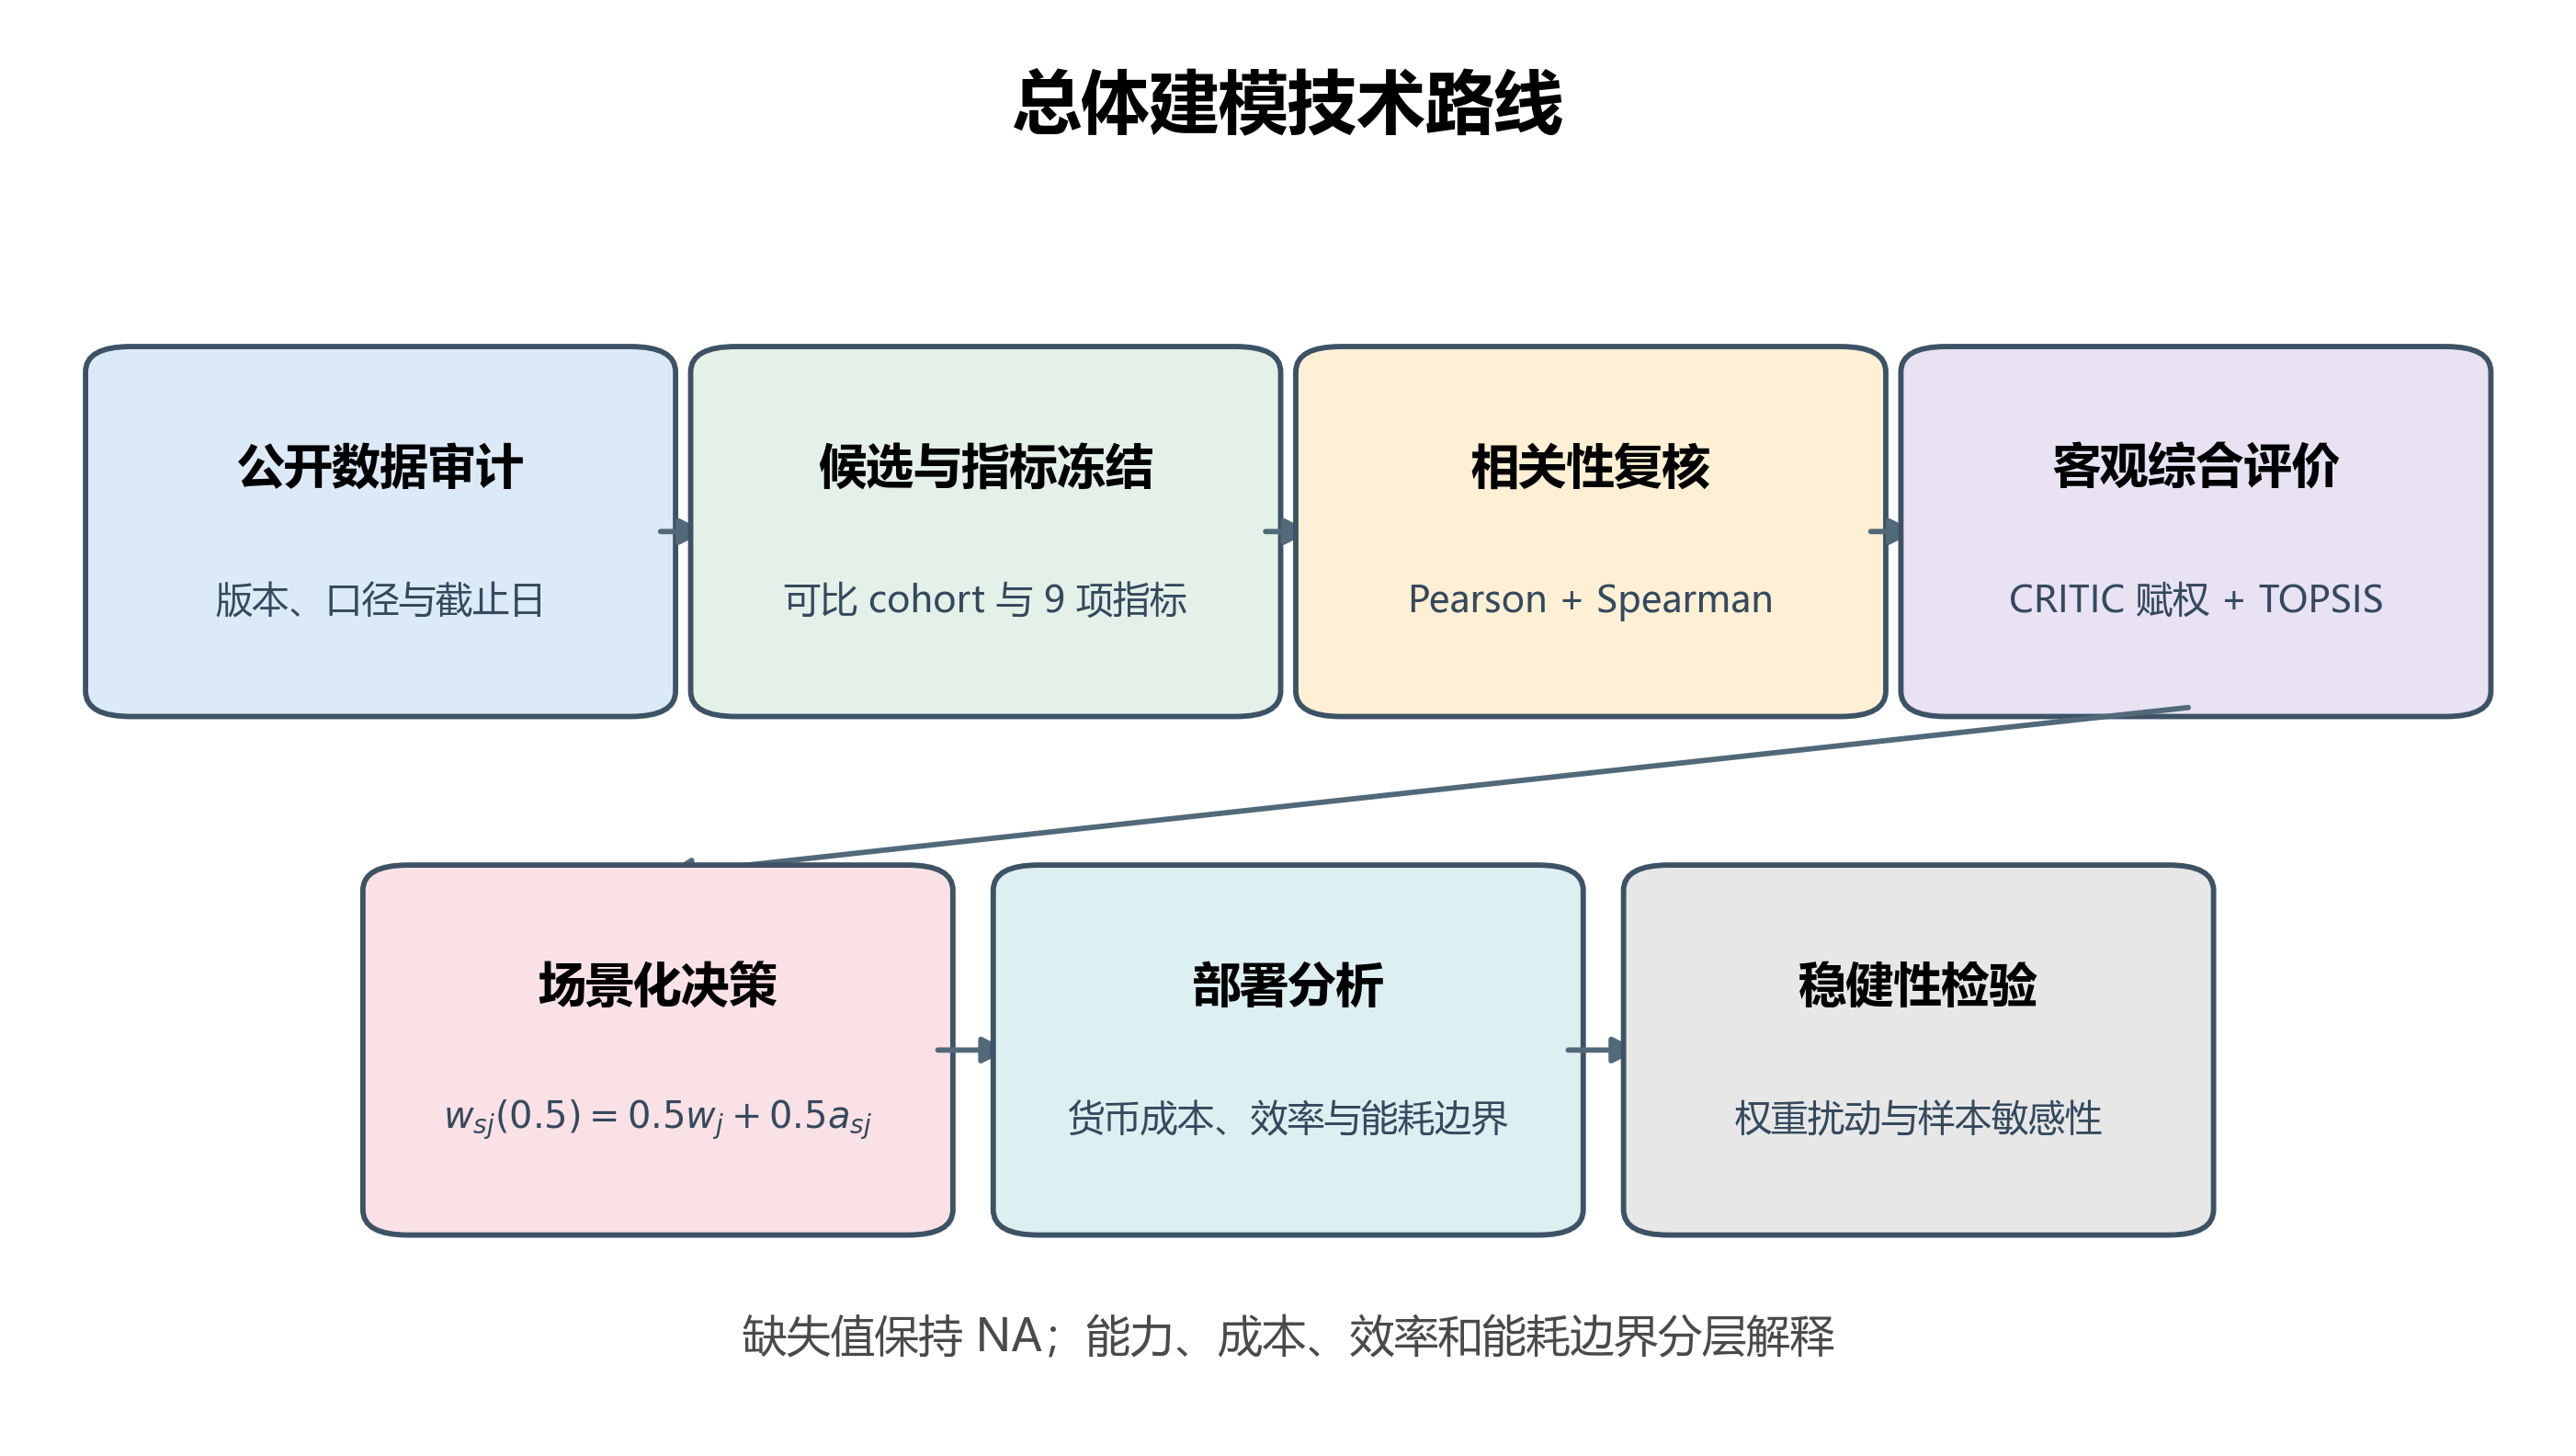
\includegraphics[width=0.90\textwidth]{tech_roadmap_enhanced.png}
  \caption{总体建模技术路线}
  \label{fig:roadmap}
\end{figure}

\subsubsection{问题一分析}

先依据可比性、覆盖率、判别力与能力语义，从候选模型和潜在指标中冻结核心评价矩阵；再用 Pearson、Spearman 相关分析识别冗余风险，以 CRITIC 确定客观权重、TOPSIS 完成综合排序，并结合分项表现分析 Kimi K3 的优势与不足。

\subsubsection{问题二分析}

针对科研长文本、大众日常对话和代码开发三类应用需求，分别设置透明的场景偏好权重，与 CRITIC 权重组合后重新进行 TOPSIS 排序；通过能力画像、加权空间及正负理想解距离解释跨场景差异，并用 $\lambda$ 敏感性检验场景结论的条件性。

\subsubsection{问题三分析}

以固定 token 工作负载下的 API 货币成本衡量直接使用成本，通过 Pareto 前沿和预算约束给出选型建议；另在严格兼容子样本中比较工程效率，审计能耗数据的可比性边界，并以小样本探索性回归描述成本与性能的样本内关系。

\section{模型假设与数据边界}

\begin{enumerate}[label=(\arabic*),leftmargin=3em]
  \item 同一冻结 cohort 内的成绩可横向比较，但不同厂商披露的最高 reasoning effort 不等价于完全相同的计算预算。
  \item 所有数据只代表 2026 年 8 月 17 日截面之前公开的信息；滚动效率观测不是模型的永久属性。
  \item 9 个核心能力指标均为效益型，数值越大表示相应能力越强。
  \item 缺失值不等于零，不进行估算、插值或任何形式的插补。
  \item 主 TOPSIS 采用 complete-case：仅对 9 项核心成绩完整的模型排序。
  \item 场景偏好权重是依据题意与应用需求作出的透明设定，不代表专家调查结果。
\end{enumerate}

\subsection{符号说明}

\begin{table}[H]
  \centering
  \small
  \caption{主要符号说明}
  \label{tab:symbols}
  \begin{tabularx}{\textwidth}{C{1.4cm}X C{1.7cm}C{1.4cm}X C{1.7cm}}
    \toprule
    符号 & 含义 & 单位 & 符号 & 含义 & 单位 \\
    \midrule
    $z_{ij}$ & 模型 $i$ 的第 $j$ 项标准化指标值 & 无量纲 &
    $w_j$ & 第 $j$ 项指标的 CRITIC 客观权重 & 无量纲 \\
    $C_j$ & 第 $j$ 项指标的 CRITIC 信息量 & 无量纲 &
    $r_{jk}$ & 指标 $j$ 与 $k$ 的 Pearson 相关系数 & 无量纲 \\
    $D_i^+$ & 模型 $i$ 到正理想解的距离 & 无量纲 &
    $D_i^-$ & 模型 $i$ 到负理想解的距离 & 无量纲 \\
    $S_i$ & 模型 $i$ 的 TOPSIS 相对贴近度 & 无量纲 &
    $a_{sj}$ & 场景 $s$ 中第 $j$ 项指标的人工偏好权重 & 无量纲 \\
    $\lambda$ & CRITIC 客观权重占比 & 无量纲 &
    $M_i$ & 模型 $i$ 在标准工作负载下的 API 货币成本 & USD \\
    $N_{\mathrm{in}}$ & 输入 token 数量 & token &
    $N_{\mathrm{out}}$ & 输出 token 数量 & token \\
    $p_{i,\mathrm{in}}$ & 模型 $i$ 的输入单价 & USD/$10^6$ tokens &
    $p_{i,\mathrm{out}}$ & 模型 $i$ 的输出单价 & USD/$10^6$ tokens \\
    \bottomrule
  \end{tabularx}
\end{table}

\section{数据来源、模型池与核心指标}

\subsection{候选模型筛选}

综合考虑模型代表性、版本明确性、公开时间、数据截止日期以及严格可比指标覆盖情况，从初始 9 个候选模型中确定 6 个最终研究对象。Gemini 3.1 Pro Preview、DeepSeek V4 Pro 0813 与 Qwen3.8 2.4T A95B 因预览状态或距数据截止日期发布时间过短、严格可比分项覆盖不足，因此不进入核心综合排名，但原始资料仍予保留。75\% 覆盖率是核心指标约束之一，并非倒推缩小模型池的唯一理由。

\begin{table}[H]
  \centering
  \caption{候选模型及冻结状态}
  \label{tab:candidates}
  \begin{tabularx}{\textwidth}{C{0.8cm}L{3.3cm}L{3.3cm}C{1.5cm}X}
    \toprule
    序号 & 模型 & 精确版本 & 状态 & 说明 \\
    \midrule
    1 & Kimi K3 & \texttt{kimi-k3} & final & 题目指定重点对象，进入核心研究池 \\
    2 & GPT-5.6 Sol & \texttt{gpt-5.6-sol} & final & 分项公开数据充分 \\
    3 & Claude Fable 5 & \texttt{claude-fable-5} & final & 能力数据充分，效率 fallback 另行排除 \\
    4 & Claude Opus 4.8 & \texttt{claude-opus-4.8} & final & 成熟对照数据充分 \\
    5 & GPT-5.5 & \texttt{gpt-5.5} & final & 稳定基线模型 \\
    6 & GLM-5.2 & \texttt{GLM-5.2} & final & 保留国产开源代表，缺失项保持 NA \\
    7 & Gemini 3.1 Pro Preview & gemini-3.1-pro-preview & excluded & preview 且严格可比覆盖不足 \\
    8 & DeepSeek V4 Pro 0813 & \texttt{DeepSeek V4 Pro 0813} & excluded & 距截止日 4 天，分项覆盖不足 \\
    9 & Qwen3.8 2.4T A95B & \texttt{Qwen3.8 2.4T A95B} & excluded & 距截止日 5 天，分项覆盖不足 \\
    \bottomrule
  \end{tabularx}
\end{table}

\subsection{潜在指标池与核心指标筛选}

为避免直接从少量熟悉的 Benchmark 中选取指标，本文先按能力构念建立潜在指标池。候选池共含 17 个概念指标：GPQA Diamond、HLE-Full、FrontierMath、MathVision、SWE-Bench Pro、DeepSWE、Terminal-Bench、FrontierSWE、SciCode、GDPval-AA v2、Agents' Last Exam、OfficeQA Pro、MMMU-Pro、OmniDocBench、CharXiv RQ、AA-LCR 与 GraphWalks BFS，覆盖高难推理、数学、代码、专业任务、多模态、文档理解和长文本等能力维度。由于 HLE-Full、MMMU-Pro、CharXiv RQ 与 MathVision 区分有无工具设置，FrontierMath 和 GraphWalks 又按难度或上下文档位拆分，17 个概念指标在覆盖率统计表中展开为 23 个 Benchmark 条目；Artificial Analysis Intelligence Index 另作模型筛选辅助，不计入这 23 项，也不进入能力综合评价。

指标筛选遵循“先可比、再覆盖、后判别与语义复核”的顺序，实际执行过程见表~\ref{tab:indicator-selection-chain}。其中，75\% 仅是覆盖率约束；来源可追溯、版本与测试设置一致、指标方向明确、具有非零变异以及能力语义不重复同样是必要条件。

\begin{table}[H]
  \centering
  \caption{潜在指标到最终核心指标的实际筛选链}
  \label{tab:indicator-selection-chain}
  \begin{tabularx}{\textwidth}{C{1.0cm}L{2.5cm}X C{1.5cm}L{2.6cm}}
    \toprule
    阶段 & 输入 & 判据 & 输出 & 处理结果 \\
    \midrule
    1 & 17 个概念指标 & 区分工具策略、难度层级与上下文档位 & 23 条 & 结构化展开；综合指数另作辅助 \\
    2 & 23 个 Benchmark 条目 & 来源、版本、测试设置与 cohort 可比，覆盖率不低于 75\% & 9 项 & 冻结核心候选；不插补、不跨口径拼接 \\
    3 & 9 项核心候选 & 正向化检查且样本标准差非零 & 9 项 & 九项均为正向能力指标且具有区分度 \\
    4 & 9 项核心候选 & $|r|$ 或 $|\rho|\geq 0.85$ 时进入冗余复核 & 4 对 & 只识别候选相关对，不自动删除 \\
    5 & 4 对候选相关对 & 综合语义维度、来源、覆盖及场景用途 & 9 项 & 删除 0 项，最终保留全部九项 \\
    \bottomrule
  \end{tabularx}
\end{table}

最终冻结 9 个核心指标。4 个指标达到 6/6 覆盖，5 个指标达到 5/6，即 83.3\%；全部达到预设的 75\% 模型覆盖要求。5 个缺失项均来自 GLM-5.2，论文不掩盖这一事实。层次上，综合评价还涉及工程效率、成本与能耗边界，但问题一的能力主排名只使用下表九项 Benchmark；工程效率与成本在问题三中另行评价，避免不同性质指标混为同一层。

\begin{table}[H]
  \centering
  \caption{最终核心指标及覆盖情况}
  \label{tab:indicators}
  \begin{tabularx}{\textwidth}{L{3.0cm}L{3.5cm}C{1.6cm}C{1.8cm}X}
    \toprule
    指标 & 维度 & 覆盖 & 覆盖率 & 缺失模型 \\
    \midrule
    GPQA Diamond & 高难科学推理 & 6/6 & 100.0\% & 无 \\
    HLE-Full（no tools） & 高难开放推理 & 5/6 & 83.3\% & GLM-5.2 \\
    AA-LCR & 长上下文推理 & 6/6 & 100.0\% & 无 \\
    SciCode & 科学编程 & 6/6 & 100.0\% & 无 \\
    GDPval-AA v2 & 专业任务 & 6/6 & 100.0\% & 无 \\
    MMMU-Pro（no tools） & 多模态推理 & 5/6 & 83.3\% & GLM-5.2 \\
    OmniDocBench & 文档理解 & 5/6 & 83.3\% & GLM-5.2 \\
    CharXiv RQ（no tools） & 科研文档推理 & 5/6 & 83.3\% & GLM-5.2 \\
    MathVision（no tools） & 多模态数学 & 5/6 & 83.3\% & GLM-5.2 \\
    \bottomrule
  \end{tabularx}
\end{table}

本文据此建立表~\ref{tab:layered-framework}所示的分层综合评价体系。问题一的 TOPSIS 得分严格定位为“通用能力核心得分”，而非混入价格、时延和能耗后的唯一终极总分。

\begin{table}[H]
  \centering
  \caption{大语言模型综合评价体系的分层结构}
  \label{tab:layered-framework}
  \begin{tabularx}{\textwidth}{L{2.2cm}L{4.1cm}X}
    \toprule
    评价层 & 指标或信息 & 在本文中的作用 \\
    \midrule
    能力性能层 & 9 项核心 Benchmark & 采用 CRITIC--TOPSIS 形成通用能力核心得分 \\
    工程效率层 & TTFT、Output Speed、500-token E2E & 仅在 4 个严格兼容模型的子样本中比较 \\
    经济成本层 & API 输入/输出价格、固定工作负载成本 & 用于性能--成本 Pareto 与预算约束选型 \\
    算力能耗层 & 理论上关注 J/token、kWh/任务等 & 完成公开数据可得性审计；不伪造量化结果 \\
    \bottomrule
  \end{tabularx}
\end{table}

四层不强行合成为单一总分：能力 Benchmark 覆盖 5 个完整排名模型，严格工程效率仅覆盖 4 个兼容模型，而能耗又缺少统一可比观测；若直接混合，将导致样本集合、测量口径和数据质量不一致。故价格与工程属性在问题三作为决策约束和落地属性分析，既覆盖综合评价要求，也避免重复计权。

\subsection{数据来源与缺失处理}

Benchmark 原始表含 148 条记录；模型元数据含 9 条模型记录及 79 条逐字段证据；效率数据含 9 条模型记录及 27 条逐指标证据。核心能力数据主要来自官方技术报告中的统一对照表，并辅以 Benchmark 榜单和独立第三方来源。每条记录保留版本、test setting、source name、URL 与检索日期；不同工具策略、agent scaffold 或快照不混入同一核心 cohort。

\begin{table}[H]
  \centering
  \caption{论文主要数据来源}
  \label{tab:main-sources}
  \begin{tabularx}{\textwidth}{L{2.1cm}L{2.7cm}X L{2.3cm}C{1.7cm}}
    \toprule
    数据类别 & 数据内容 & 主要来源 & 来源类型 & 检索日期 \\
    \midrule
    能力 Benchmark & 9 项核心成绩 & Kimi K3 Technical Report；OpenAI 与 Z.ai 官方报告作辅助证据\cite{kimi-k3,openai-launch,zai-launch} & 厂商官方报告 & 2026-08-16/17 \\
    模型身份 & provider、exact version、发布日期 & Moonshot、OpenAI、Anthropic 与 Z.ai 官方模型资料\cite{kimi-blog,openai-models,anthropic-models,zai-launch} & 第一方官方文档 & 2026-08-16/17 \\
    API 价格 & 输入、输出标准价 & 模型厂商官方定价页面\cite{openai-pricing,anthropic-pricing,zhipu-pricing} & 第一方定价文档 & 2026-08-16/17 \\
    部署效率 & TTFT、Output Speed、E2E & Artificial Analysis API Provider Performance Benchmarking\cite{aa} & 独立评测平台 & 2026-08-16 \\
    能耗边界 & 可得性与可比性 & 对模型官方资料、公开定价资料及独立评测数据的可得性审计 & 公开数据审计 & 2026-08-17 \\
    \bottomrule
  \end{tabularx}
\end{table}

冻结的 9 项核心成绩均主要采用 Kimi K3 Technical Report 的统一 cohort，以保持测试设置一致。OpenAI、Z.ai 官方报告、Benchmark 官方资料和 Artificial Analysis 等作为辅助来源证据，但不替换冻结 cohort，也不宣称已完成独立交叉验证。数据整理时逐条记录来源 URL、比较口径和检索日期，以保证核心数字可追溯。

\noindent\textit{AI 使用标注：本节的数据来源一致性检查与数据核验使用了 AI 工具辅助，最终数据取舍、缺失值保留和截止日期均由参赛队人工确认，详见支撑材料《人工智能工具使用详情》。}

Raw 层缺失统一保持为 NA。描述统计与 Pearson、Spearman 相关性采用逐对完整观测；主 TOPSIS 采用 complete-case。GLM-5.2 只有 4/9 项核心成绩，因此不进入主排名。本文没有将缺失值写为零，也没有进行跨来源平均、擅自取最大值或任何形式的插补。

不同量纲指标采用效益型极差标准化：
\begin{equation}
  z_{ij}=\frac{x_{ij}-\min_i x_{ij}}{\max_i x_{ij}-\min_i x_{ij}}.
  \label{eq:minmax}
\end{equation}

标准化在每项指标内部独立完成，因此百分制、Elo 等不同原始量纲不直接相加，而是统一转换为当前候选集合内的相对位置。若某指标仅有 5 个满足同口径要求的有效观测，则该指标的最大值与最小值仅由这 5 个有效模型确定，缺失模型不参与极值计算。

\section{问题一：CRITIC--TOPSIS 综合评价}

\subsection{相关性与指标保留}

9 个指标的标准差均非零。本文同时计算逐对完整观测上的 Pearson 系数 $r$ 与 Spearman 系数 $\rho$，并将 $|r|$ 或 $|\rho|\geq0.85$ 设为高相关候选的冗余审查阈值；该阈值仅用于触发后续语义复核，并非统计显著性检验阈值。由于共同观测模型仅为 5--6 个，本文不依据相关系数进行总体参数显著性推断。由此得到 4 组候选对：GPQA Diamond--MMMU-Pro（$r=0.9500,\ \rho=0.9211$）、GPQA Diamond--MathVision（$r=0.8611,\ \rho=0.6669$）、SciCode--CharXiv RQ（$r=0.9326,\ \rho=0.9747$）以及 MMMU-Pro--MathVision（$r=0.9349,\ \rho=0.8208$），共同观测量均为 $n=5$。这些关系只表明当前小样本内存在较高线性或秩相关，是冗余判断的辅助证据，并不能证明指标语义等价。前置筛选已将 17 个概念指标展开为 23 个条目，再按可比性、覆盖率与判别力缩减至 9 项；相关性分析的作用是对最终候选进行冗余风险检查，而非机械继续压缩数量。综合覆盖率、来源口径、能力构念和后续场景用途复核后，高相关指标仍测量不同能力构念并承担不同场景解释作用，故 4 组候选对均保留；删除 0 项表示相关性经语义与场景信息复核后尚不足以支持删项，而非相关性分析无效。

图~\ref{fig:pearson} 直观展示 Pearson 相关结构；Spearman 结果仍按正文所述共同参与冗余复核。
\begin{figure}[htbp]
  \centering
  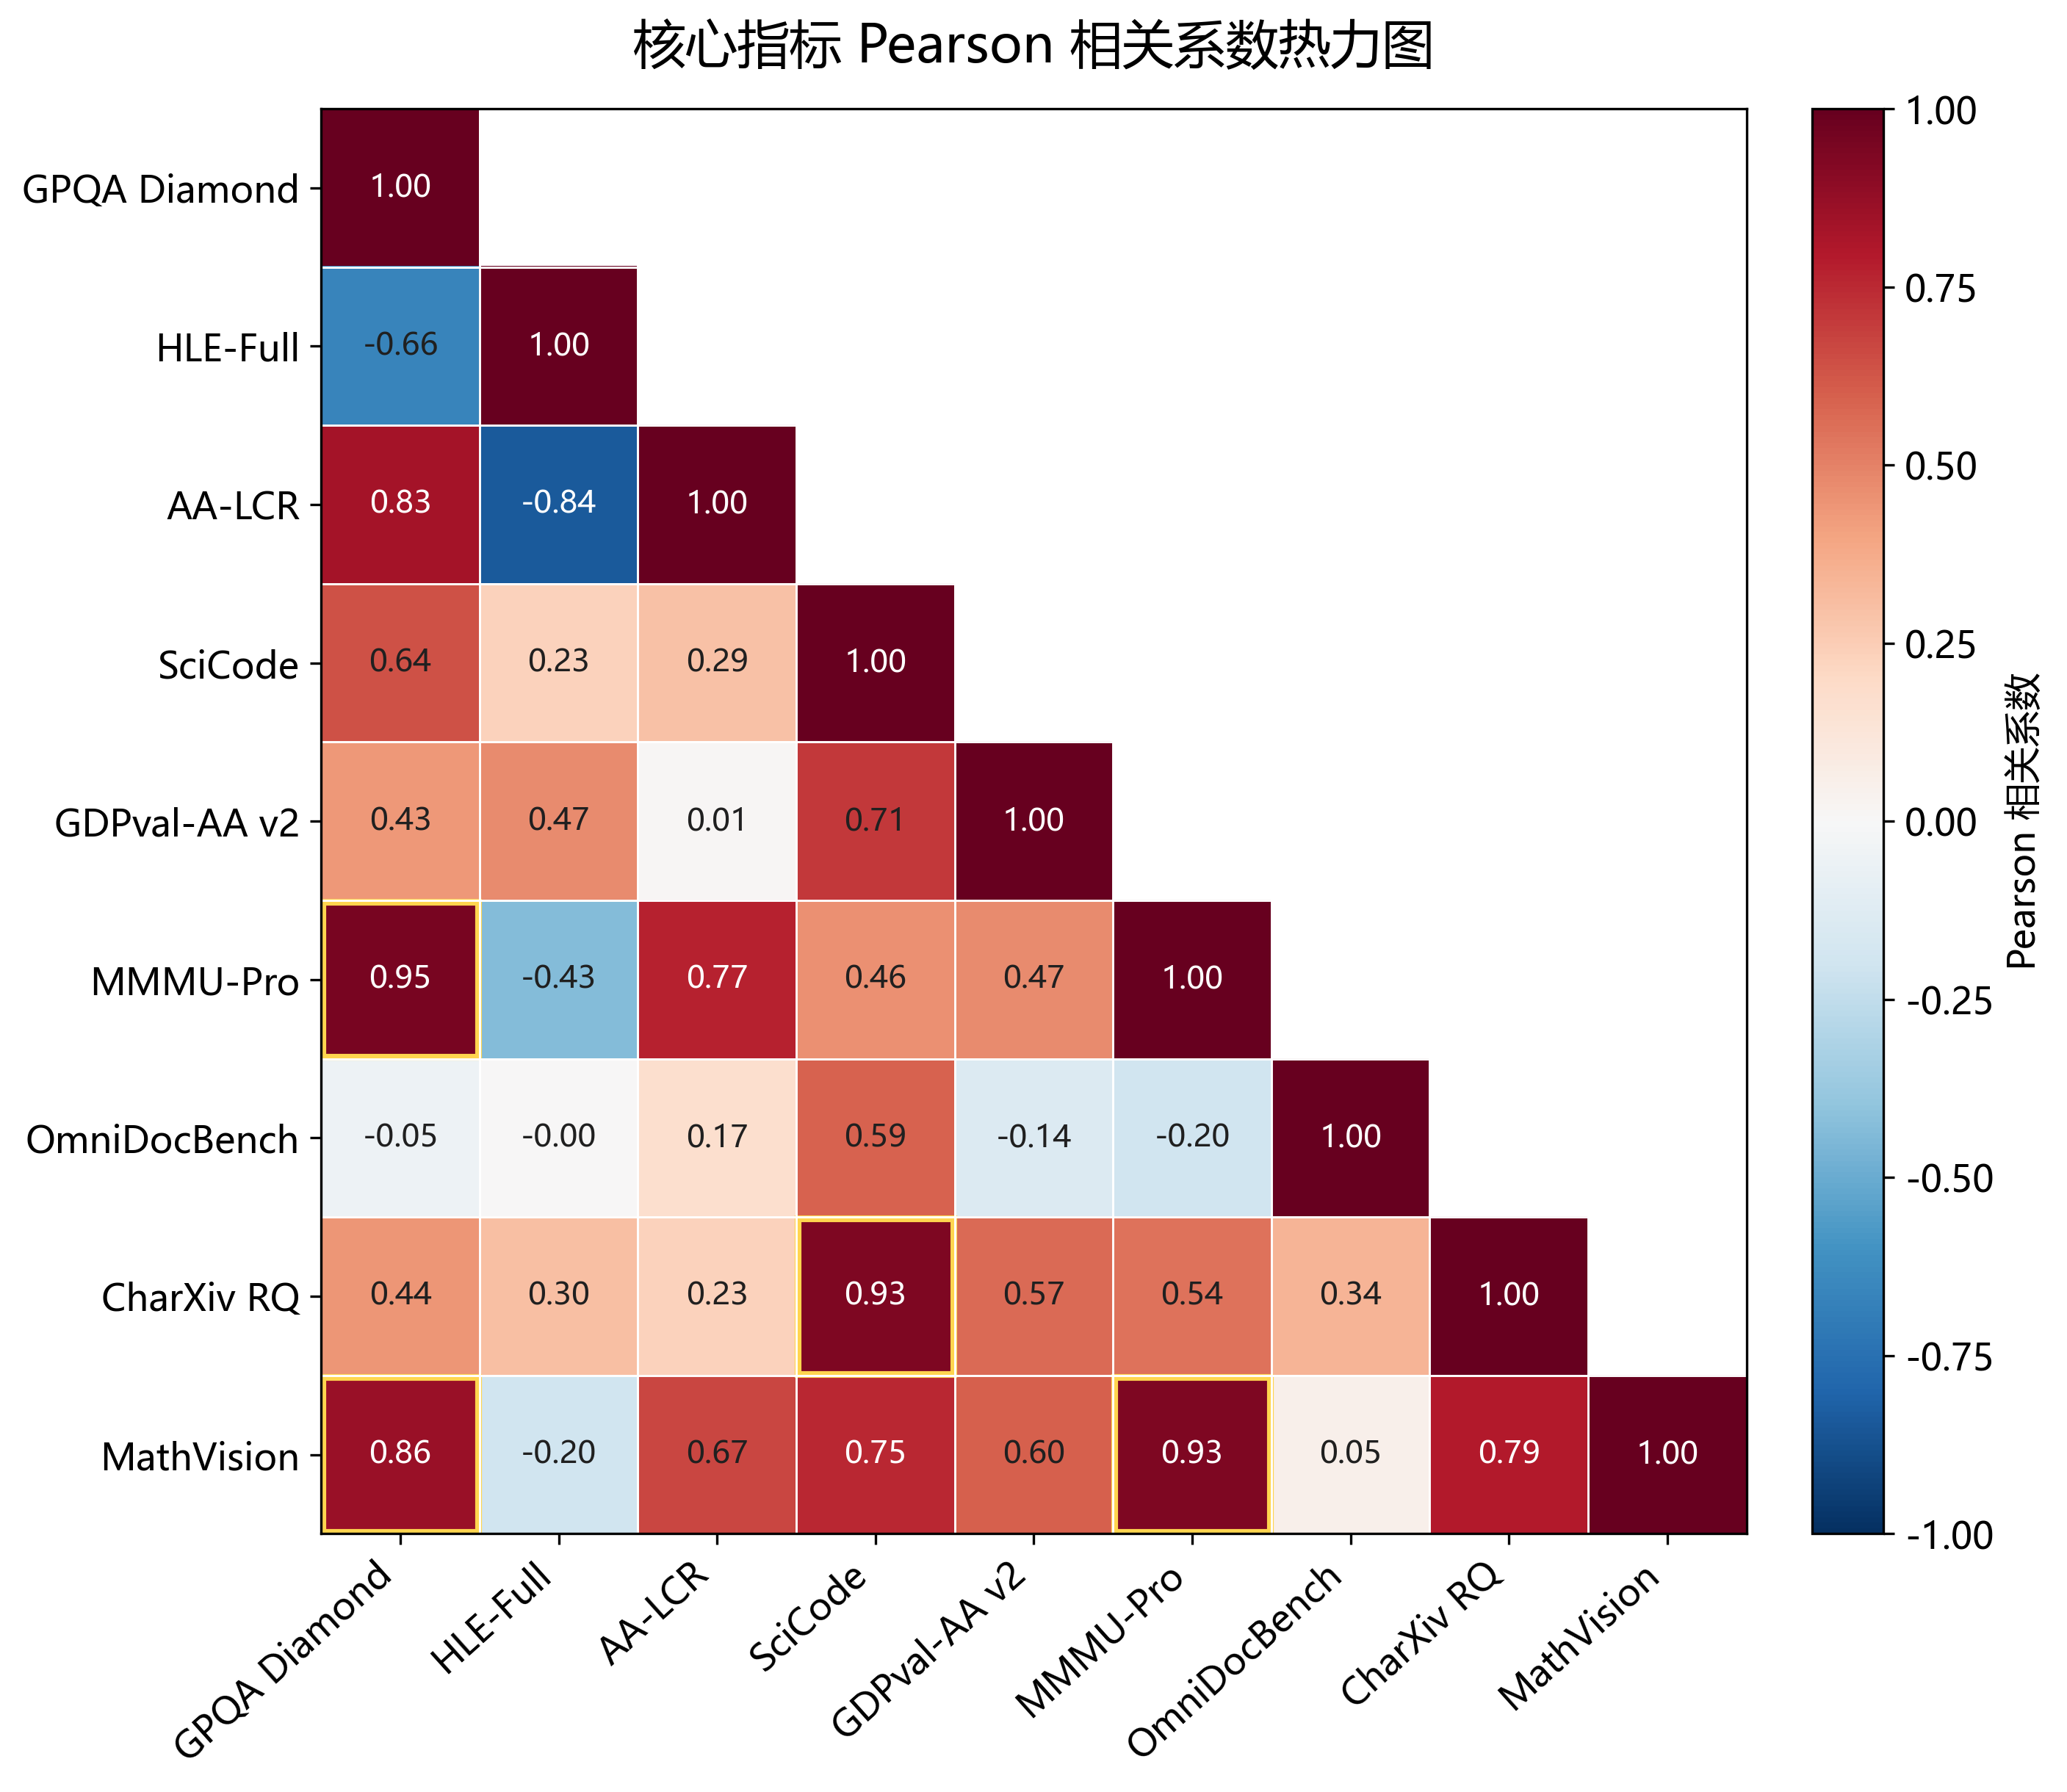
\includegraphics[width=0.76\textwidth]{pearson_heatmap_enhanced.png}
  \caption{核心指标 Pearson 相关系数热力图}
  \label{fig:pearson}
\end{figure}

\subsection{CRITIC 客观赋权}

本文选择 CRITIC，是因为九项指标均为客观公开 Benchmark 结果，且需要同时利用指标的样本变异性与指标间冲突性，减少主权重完全依赖主观判断。AHP 需要真实专家判断矩阵，本研究未实施专家调查，故不将其用作主权重；熵权法主要依赖离散程度，本文将其保留为稳健性对照且所得排名一致；PCA 更强调降维和线性组合，其主成分不如原始 Benchmark 权重便于解释。因此，CRITIC 与本题存在相关结构且强调可解释客观赋权的需求更匹配。

\noindent\textit{AI 使用标注：相关程序实现与调试使用了 AI 代码辅助工具；模型公式、参数、输入数据和最终计算结果均由参赛队复核。}

CRITIC 方法同时利用标准化指标的变异性和指标间冲突性\cite{critic}。令第 $j$ 个指标的总体标准差为 $\sigma_j$，逐对完整观测上的 Pearson 相关系数为 $r_{jk}$，则
\begin{equation}
  C_j=\sigma_j\sum_{k=1}^{n}(1-r_{jk}),\qquad
  w_j=\frac{C_j}{\sum_{j=1}^{n}C_j}.
  \label{eq:critic}
\end{equation}

\begin{table}[H]
  \centering
  \caption{CRITIC 最终权重}
  \label{tab:critic}
  \begin{tabularx}{0.82\textwidth}{L{4.5cm}C{2.5cm}X}
    \toprule
    指标 & 权重 & 权重排序 \\
    \midrule
    GPQA Diamond & 0.1039 & 5 \\
    HLE-Full & 0.2013 & 1 \\
    AA-LCR & 0.1270 & 3 \\
    SciCode & 0.0674 & 9 \\
    GDPval-AA v2 & 0.1167 & 4 \\
    MMMU-Pro & 0.0865 & 6 \\
    OmniDocBench & 0.1483 & 2 \\
    CharXiv RQ & 0.0734 & 8 \\
    MathVision & 0.0756 & 7 \\
    \bottomrule
  \end{tabularx}
\end{table}

HLE-Full、OmniDocBench 与 AA-LCR 权重依次居前三，SciCode 权重最低。权重反映当前样本中的变异性与冲突性，不等同于脱离样本和场景的绝对重要程度。

\begin{figure}[H]
  \centering
  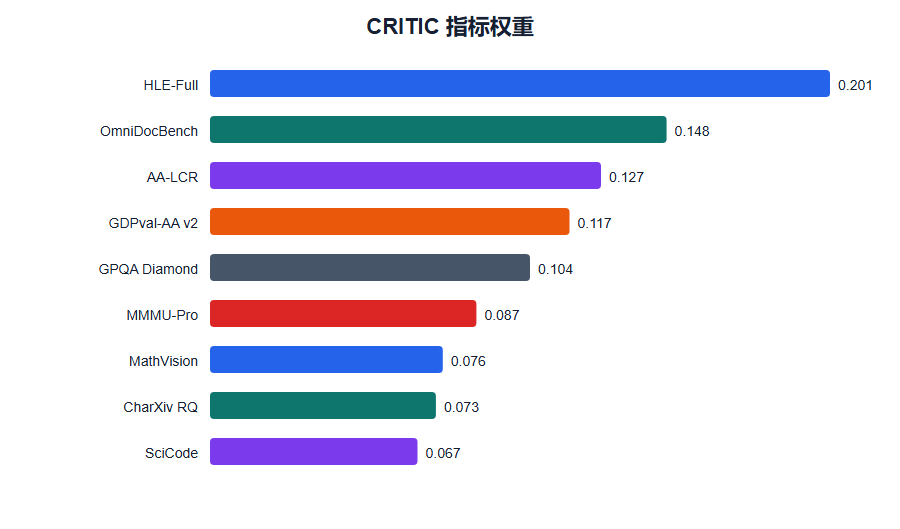
\includegraphics[width=0.86\textwidth]{critic_weights.png}
  \caption{CRITIC 指标权重}
  \label{fig:critic}
\end{figure}

\subsection{TOPSIS 综合评价}

TOPSIS 以模型到正、负理想解的距离刻画相对贴近程度\cite{topsis}。首先构造加权标准化矩阵：
\begin{equation}
  v_{ij}=w_jz_{ij}.
  \label{eq:weighted-matrix}
\end{equation}
正、负理想解为
\begin{equation}
  v_j^+=\max_i v_{ij},\qquad v_j^-=\min_i v_{ij}.
\end{equation}
模型到两个理想解的欧氏距离为
\begin{align}
  D_i^+&=\sqrt{\sum_{j=1}^{n}(v_{ij}-v_j^+)^2},\\
  D_i^-&=\sqrt{\sum_{j=1}^{n}(v_{ij}-v_j^-)^2}.
\end{align}
相对贴近度为
\begin{equation}
  S_i=\frac{D_i^-}{D_i^++D_i^-}.
  \label{eq:topsis}
\end{equation}
式~\eqref{eq:weighted-matrix}--\eqref{eq:topsis}与程序实际使用的加权矩阵和距离完全一致。

\begin{table}[H]
  \centering
  \caption{通用能力 TOPSIS 核心得分与排名}
  \label{tab:topsis}
  \begin{tabularx}{0.86\textwidth}{C{1.3cm}L{4.3cm}C{2.5cm}X}
    \toprule
    排名 & 模型 & TOPSIS 得分 & 状态 \\
    \midrule
    1 & Claude Fable 5 & 0.7254 & 完整样本排名 \\
    2 & Kimi K3 & 0.5933 & 完整样本排名 \\
    3 & GPT-5.6 Sol & 0.5178 & 完整样本排名 \\
    4 & GPT-5.5 & 0.4410 & 完整样本排名 \\
    5 & Claude Opus 4.8 & 0.3902 & 完整样本排名 \\
    -- & GLM-5.2 & NA & 4/9，数据不足不排名 \\
    \bottomrule
  \end{tabularx}
\end{table}

\begin{figure}[H]
  \centering
  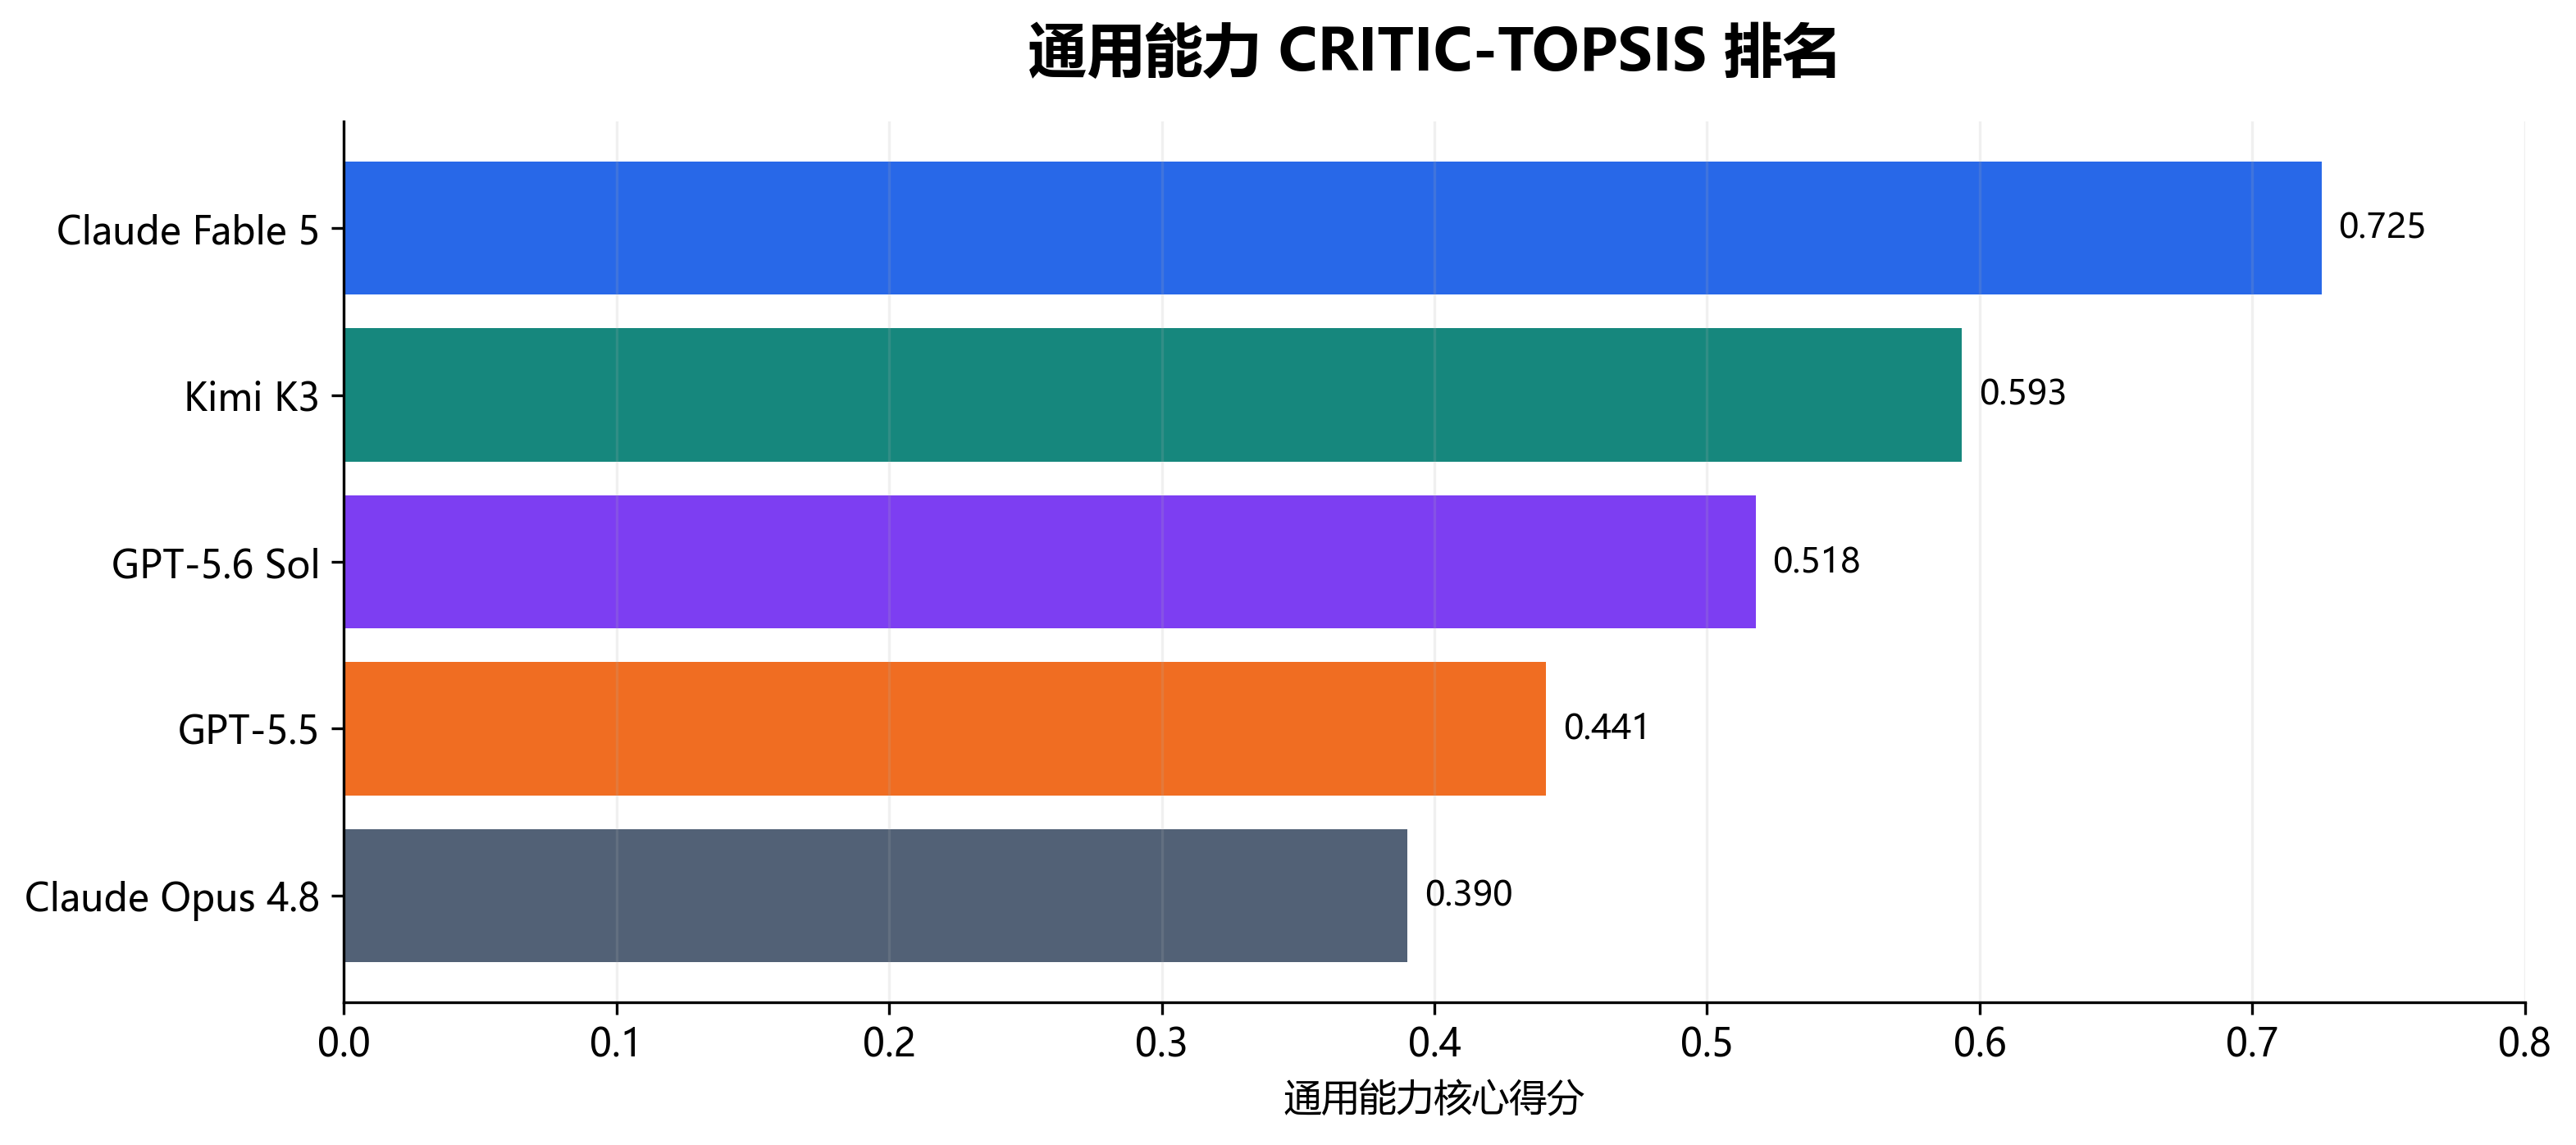
\includegraphics[width=0.86\textwidth]{general_ranking.png}
  \caption{通用能力综合排名}
  \label{fig:ranking}
\end{figure}

Kimi K3 在 AA-LCR 与 OmniDocBench 上排名第一，在 GPQA Diamond、SciCode 和 MMMU-Pro 上排名第二，优势集中在长上下文、文档理解、高难科学推理与科学编程；GDPval-AA v2、CharXiv RQ 与 MathVision 分别处于第 3、第 2和第 3，体现其专业任务、科研图表和多模态数学能力处于中上位置。其 HLE-Full 标准化得分为 0.1765，在 5 个完整模型中位列第 4，是最明确的能力短板。场景上，Kimi 在 $\lambda=0.5$ 的科研长文本场景排名第一，在日常对话和代码开发场景均排名第二，且科研榜首具有 $\lambda$ 条件性；成本上其标准工作负载为 6 美元并位于 Pareto 前沿。严格效率结论仅依据 4 模型兼容子样本，不使用 Fable 或 GLM 的不兼容观测作横向推断。

图~\ref{fig:kimi-radar} 将 9 项核心指标按冻结能力维度映射为 8 个能力画像维度，其中高难度知识与逻辑推理由 GPQA Diamond 和 HLE-Full 按其 CRITIC 权重在维度内归一聚合，其余维度各对应一项核心指标。该图仅用于描述完整样本中的能力画像，不参与 CRITIC 赋权或 TOPSIS 排名。
\begin{figure}[htbp]
  \centering
  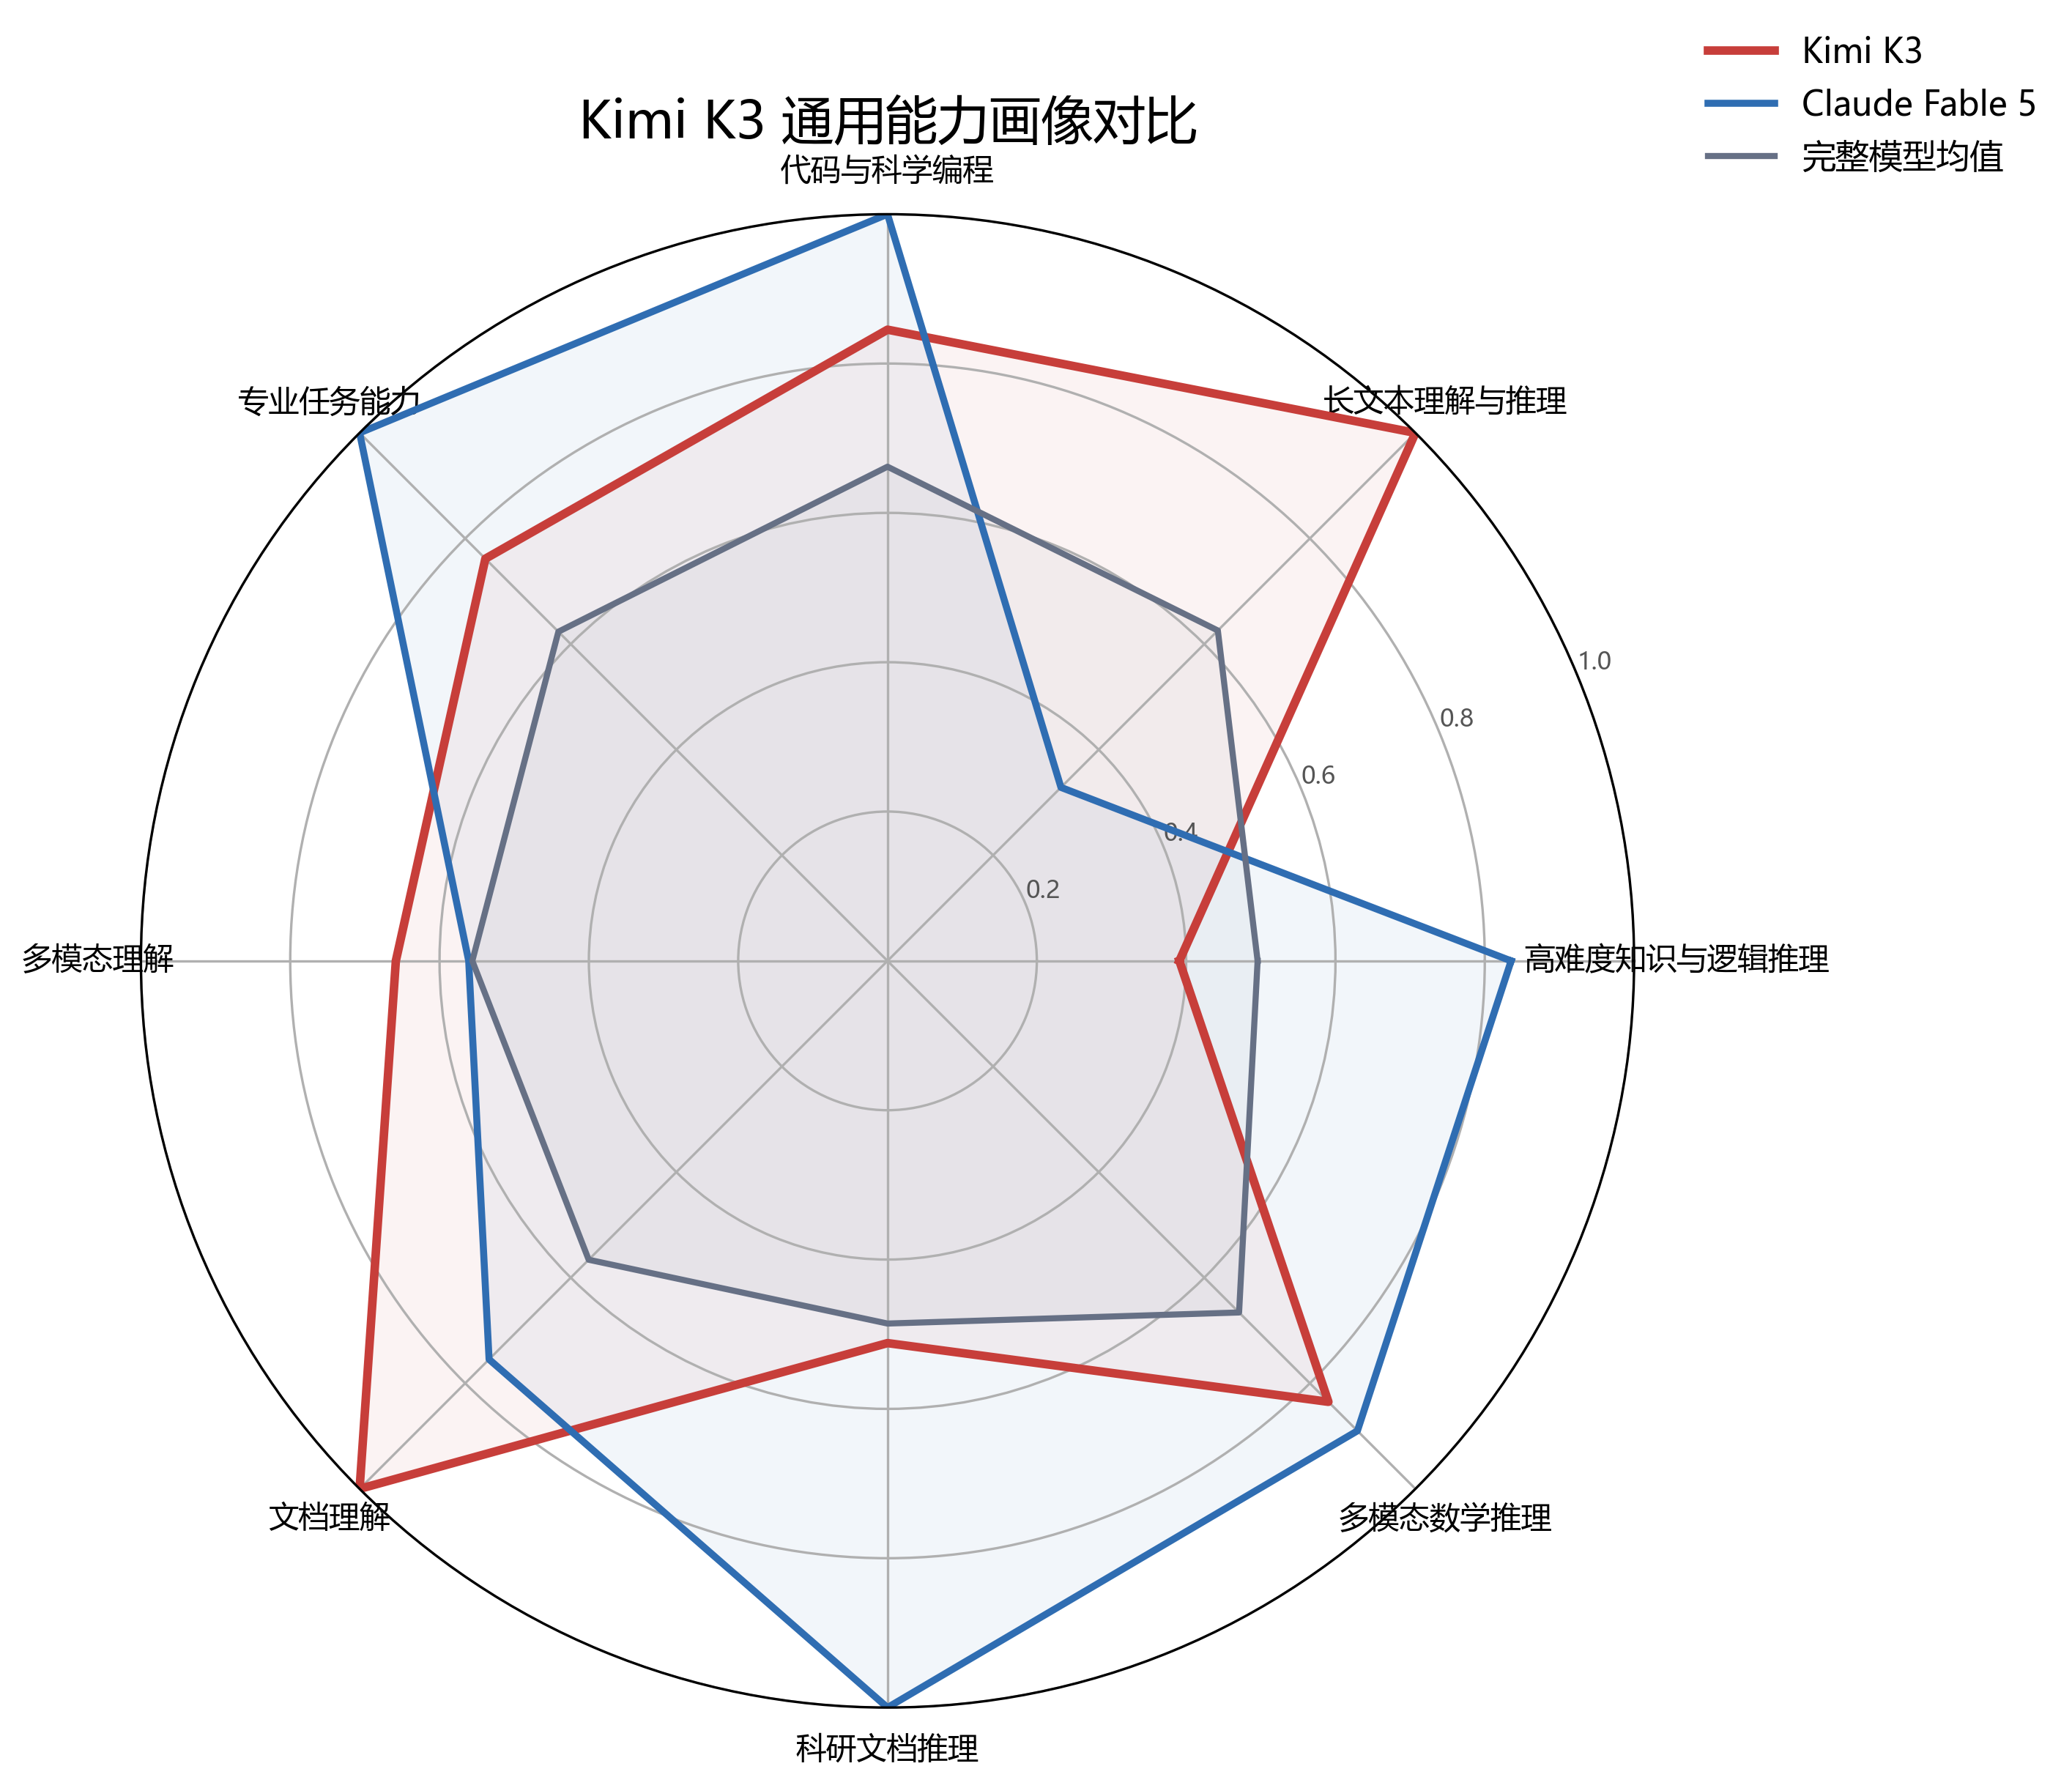
\includegraphics[width=0.78\textwidth]{kimi_k3_ability_radar.png}
  \caption{Kimi K3 通用能力画像对比}
  \label{fig:kimi-radar}
\end{figure}

\paragraph{GLM-5.2 局部观察。}基于四项共同可观测指标的局部比较结果显示，在六模型共同有观测的 GPQA Diamond、AA-LCR、SciCode 与 GDPval-AA v2 上，GLM-5.2 分别位列第 5、第 4、第 6和第 5；其相对各指标领先模型的差距依次为 2.9 个百分点、3.4 个百分点、9.7 个百分点和 237 Elo。该比较仅用于描述共同观测维度，不构成九项完整综合得分，也不用于推断 GLM-5.2 的主排名；其余 5 项缺失仍保持 NA，不进行插补。

另据 Z.ai 官方资料，GLM-5.2 的独立 HLE 成绩为 40.5，但其测试来源与本文冻结 cohort 不一致，因此仅作为补充证据，不用于替换主矩阵中的 HLE 缺失值\cite{zai-launch}。

\section{问题二：三类场景评价}

\subsection{场景权重构造}

对场景 $s$，令 $a_{sj}$ 为依据题意与应用需求设定的人工场景偏好，$\lambda$ 为 CRITIC 客观权重占比，则组合权重为
\begin{equation}
  w_{sj}(\lambda)=\lambda w_j+(1-\lambda)a_{sj}.
  \label{eq:scenario-weight}
\end{equation}
本文以 $\lambda=0.5$ 作为正式基准，即对 CRITIC 客观信息与题意驱动的场景偏好给予等比例组合。该取值用于构造透明、易解释的基准场景，并非由优化程序或专家调查得到的唯一最优比例。三组 $a_{sj}$ 与 $w_{sj}(0.5)$ 均非负且和为 1；本文没有实施专家调查，因此不将 $a_{sj}$ 称为专家权重。使用 $w_{sj}(0.5)$ 替代通用 CRITIC 权重后，按照式~\eqref{eq:weighted-matrix}--\eqref{eq:topsis}重新计算场景 TOPSIS 得分。

表~\ref{tab:scenario-preferences}列出正式人工场景偏好 $a_{sj}$。这些数值依据赛题定义的应用需求与各指标能力语义进行透明的规则化设定：科研长文本突出长上下文、科研文档与高难推理；日常对话更重视专业任务泛化、多模态理解与任务均衡；代码开发显著提高与科学编程直接相关的 SciCode。它们属于场景先验而非统计估计量，故本文进一步以 $\lambda$ 敏感性分析检验其对结论的影响。

\begin{table}[H]
  \centering
  \caption{三类场景人工偏好权重设定}
  \label{tab:scenario-preferences}
  \begin{tabularx}{0.90\textwidth}{L{4.0cm}C{2.2cm}C{2.2cm}X}
    \toprule
    指标 & 科研长文本 $a_{sj}$ & 日常对话 $a_{sj}$ & 代码开发 $a_{sj}$ \\
    \midrule
    GPQA Diamond & 0.12 & 0.12 & 0.12 \\
    HLE-Full & 0.12 & 0.12 & 0.08 \\
    AA-LCR & 0.25 & 0.10 & 0.08 \\
    SciCode & 0.05 & 0.03 & 0.40 \\
    GDPval-AA v2 & 0.08 & 0.20 & 0.12 \\
    MMMU-Pro & 0.08 & 0.15 & 0.05 \\
    OmniDocBench & 0.12 & 0.10 & 0.05 \\
    CharXiv RQ & 0.13 & 0.06 & 0.05 \\
    MathVision & 0.05 & 0.12 & 0.05 \\
    \midrule
    合计 & 1.00 & 1.00 & 1.00 \\
    \bottomrule
  \end{tabularx}
\end{table}

正式最终场景权重不另行人为设定，而是由 $w_{sj}(0.5)=0.5w_j+0.5a_{sj}$ 计算得到。

三类场景的最终组合权重如图~\ref{fig:scenario-weights} 所示，其中展示的是 $w_{sj}(0.5)$，而非人工偏好 $a_{sj}$。
\begin{figure}[H]
  \centering
  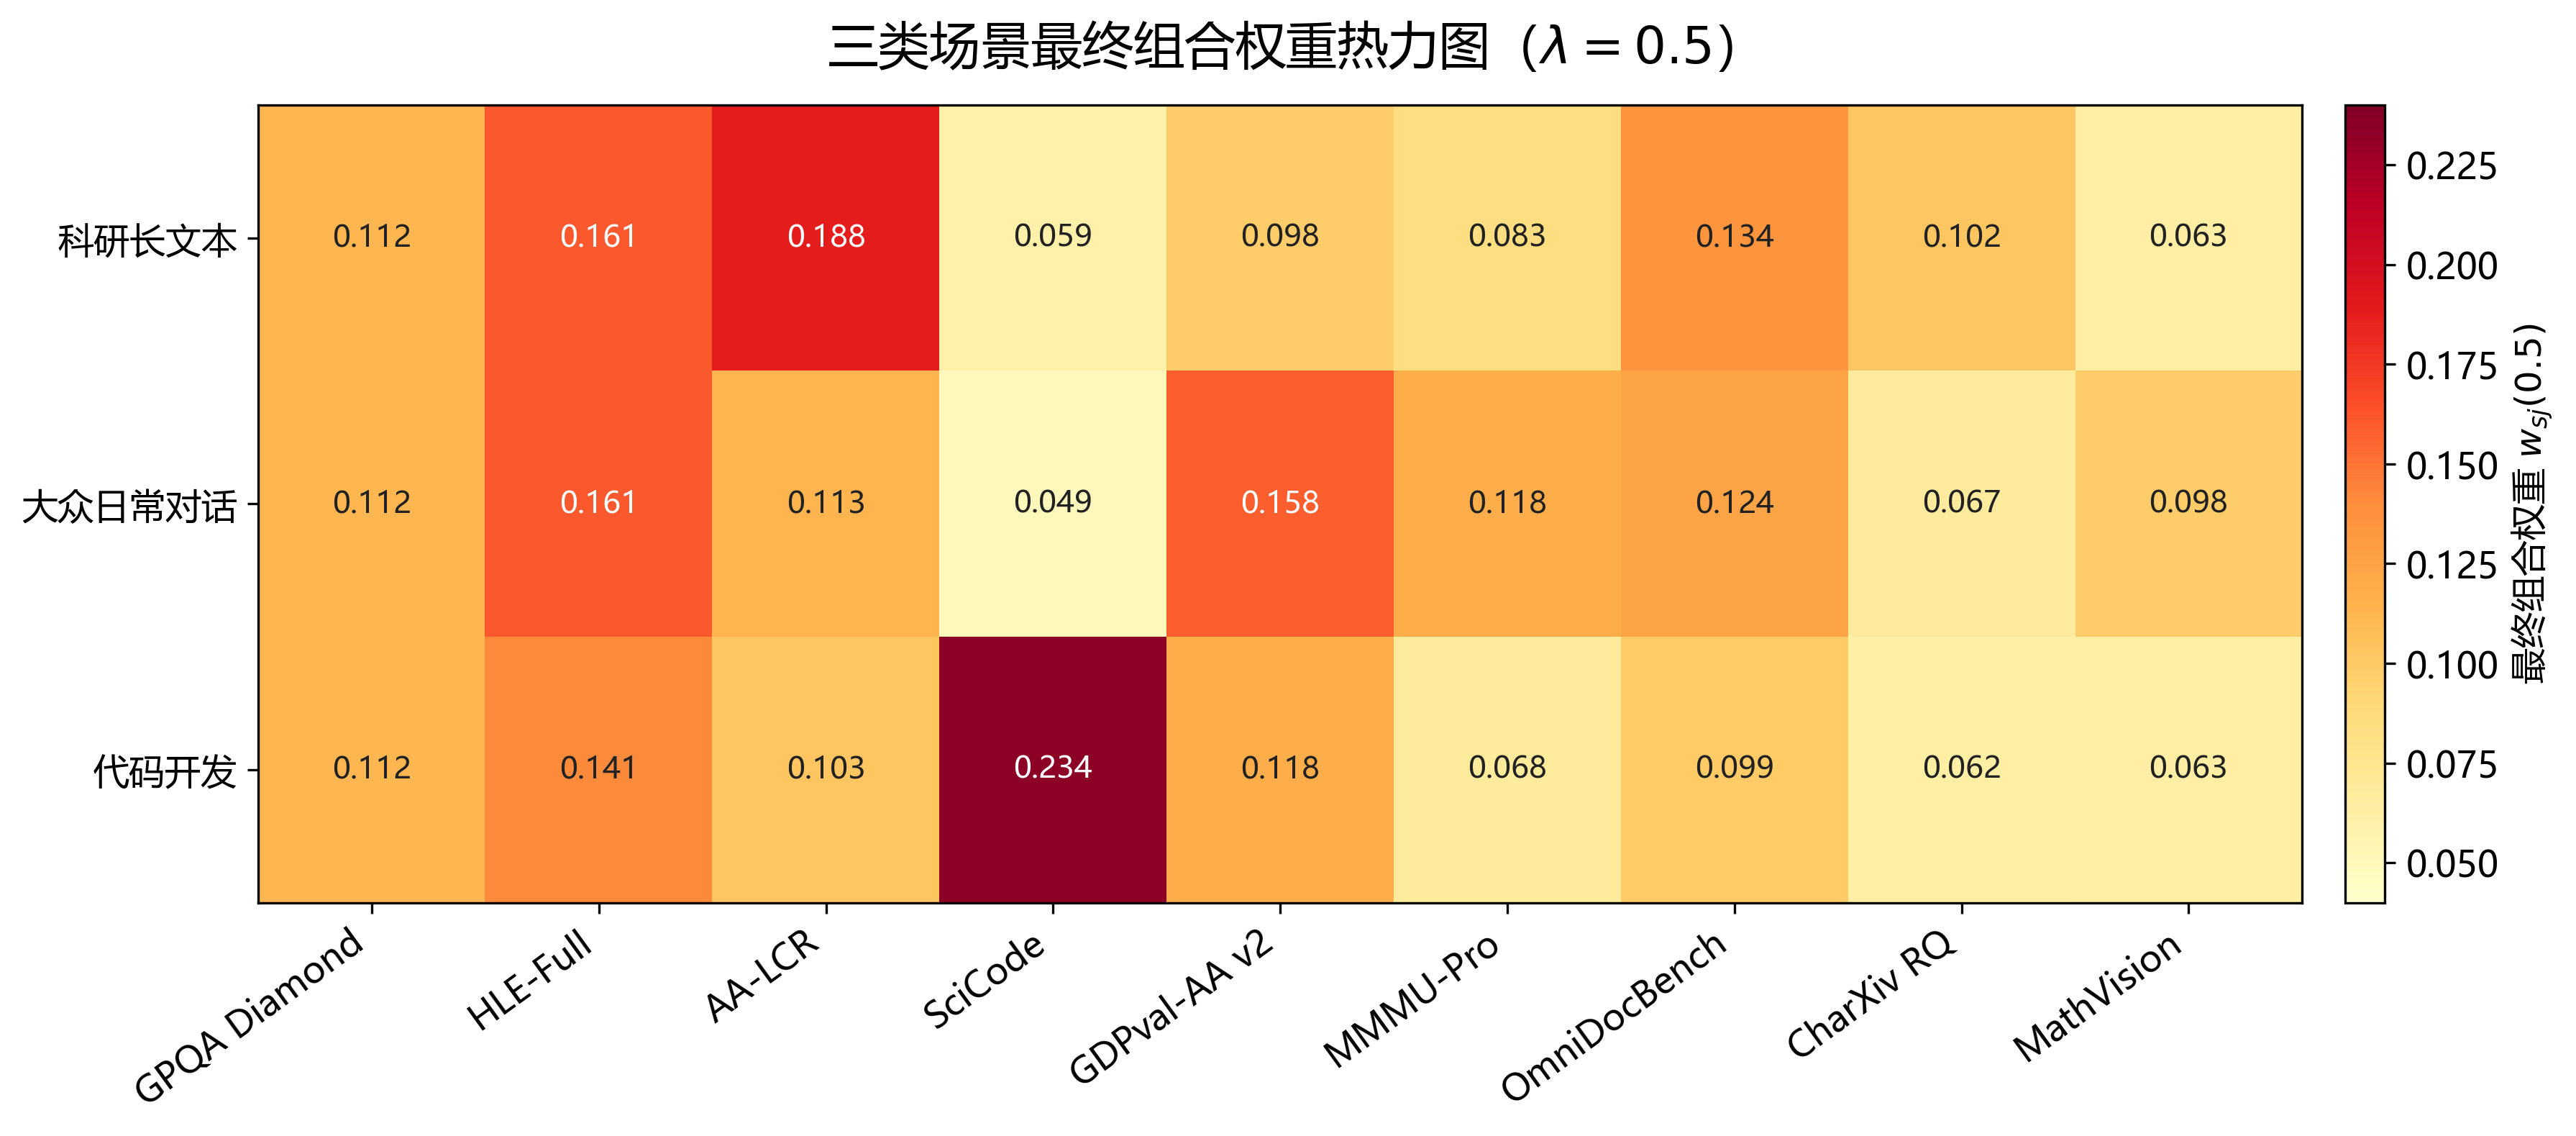
\includegraphics[width=0.90\textwidth]{scenario_weights_heatmap_enhanced.png}
  \caption{三类场景最终组合权重热力图（$\lambda=0.5$）}
  \label{fig:scenario-weights}
\end{figure}

\begin{table}[H]
  \centering
  \caption{三类场景完整排名与得分}
  \label{tab:scenarios}
  \begin{tabularx}{\textwidth}{L{2.7cm}C{1.0cm}L{3.3cm}C{2.2cm}X}
    \toprule
    场景 & 排名 & 模型 & 场景得分 & 相对通用排名 \\
    \midrule
    \multirow{5}{*}{科研长文本}
      & 1 & Kimi K3 & 0.6547 & 上升 1 位 \\
      & 2 & Claude Fable 5 & 0.6471 & 下降 1 位 \\
      & 3 & GPT-5.6 Sol & 0.5703 & 不变 \\
      & 4 & GPT-5.5 & 0.5276 & 不变 \\
      & 5 & Claude Opus 4.8 & 0.3147 & 不变 \\
    \midrule
    \multirow{5}{*}{大众日常对话}
      & 1 & Claude Fable 5 & 0.7208 & 不变 \\
      & 2 & Kimi K3 & 0.6343 & 不变 \\
      & 3 & GPT-5.6 Sol & 0.6024 & 不变 \\
      & 4 & GPT-5.5 & 0.4392 & 不变 \\
      & 5 & Claude Opus 4.8 & 0.3431 & 不变 \\
    \midrule
    \multirow{5}{*}{代码开发}
      & 1 & Claude Fable 5 & 0.7722 & 不变 \\
      & 2 & Kimi K3 & 0.6840 & 不变 \\
      & 3 & GPT-5.6 Sol & 0.5838 & 不变 \\
      & 4 & GPT-5.5 & 0.4896 & 不变 \\
      & 5 & Claude Opus 4.8 & 0.3384 & 不变 \\
    \bottomrule
  \end{tabularx}
\end{table}

\begin{figure}[H]
  \centering
  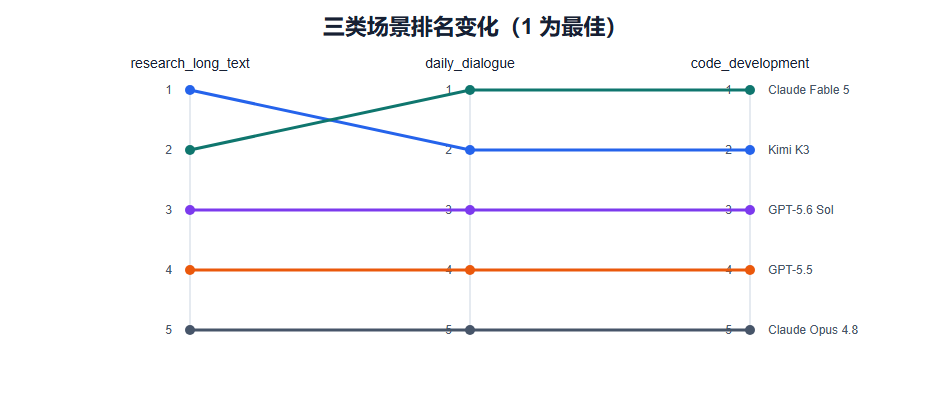
\includegraphics[width=0.90\textwidth]{scenario_rank_changes.png}
  \caption{三类场景排名变化}
  \label{fig:scenario}
\end{figure}

在 $\lambda=0.5$ 的基准组合下，科研长文本场景提高了 AA-LCR、CharXiv RQ 和 GPQA Diamond 等指标的权重作用，使 Kimi K3 从通用第 2 升至第 1。日常对话与代码开发中 Claude Fable 5 保持第一，Kimi K3 保持第二。组合系数敏感性分析进一步表明，科研长文本榜首在离散测试网格的 $\lambda=0.5$ 与 $0.6$ 之间发生 Kimi K3 与 Claude Fable 5 的切换，故该榜首结论应理解为基准设定下的条件性结果。GLM-5.2 仍因核心矩阵不完整而不进入场景 TOPSIS 排名。

\subsection{跨场景排名差异的内在机理}

模型 $i$ 的九维标准化能力画像 $\bm z_i=(z_{i1},\ldots,z_{in})$ 不随场景改变；变化的是场景权重向量 $\bm w_s$。对同一能力画像进行 $v_{isj}=w_{sj}z_{ij}$ 加权后，模型在加权标准化空间中的位置随场景需求而改变，进而改变其到正、负理想解的距离 $D_i^+$、$D_i^-$ 以及 TOPSIS 贴近度。因此，跨场景排名差异不是模型基础能力突然变化，而是同一能力画像在不同需求权重下被重新评价。下文提及的指标作用只描述能力差异与权重结构的方向性匹配，不将其称为单项 TOPSIS 得分贡献。

科研长文本场景的核心是两种能力结构的强对冲。相对 Claude Fable 5，Kimi K3 在 AA-LCR、GPQA Diamond 和 OmniDocBench 上的标准化优势分别为 0.6714、0.2903 和 0.2453；Fable 则在 HLE-Full、CharXiv RQ 和 GDPval-AA v2 上分别领先 0.8235、0.4881 和 0.2383。基准场景相对通用 CRITIC 权重重点提高 AA-LCR，并降低 HLE-Full 与 GDPval-AA v2 的权重作用，使 Kimi 的长文本和科学推理优势得到更充分体现，但未消除 Fable 在极高难推理和科研图文理解上的优势。在 $\lambda=0.5$ 时，Kimi 的 $D^+=0.148272$ 略大于 Fable 的 0.146343，即 Kimi 并非更接近正理想解；但其 $D^-=0.281092$ 大于 Fable 的 0.268320，整体更远离负理想解。两种距离共同作用后，Kimi 以 0.654670 对 0.647080 小幅领先，差距仅为 0.007590。

当科研场景的 $\lambda$ 由 0.5 增至 0.6 时，CRITIC 客观权重作用增强而定向场景偏好减弱。Kimi 最主要的 AA-LCR 优势权重下降，同时 HLE-Full 权重回升，进一步体现 Fable 的相对优势；CharXiv RQ 权重下降与 OmniDocBench 权重上升对 Kimi 形成一定反向补偿，但不足以抵消前两项变化。对应的距离结构中，Kimi 的 $D^+$ 由 0.148272 增至 0.153590，$D^-$ 由 0.281092 降至 0.275137；Fable 的 $D^+$ 由 0.146343 降至 0.139215，$D^-$ 由 0.268320 增至 0.273219。于是 Kimi 的贴近度降至 0.641754，Fable 升至 0.662454，与离散网格上 $[0.5,0.6]$ 内出现的榜首切换一致。

大众日常对话场景主要提高 GDPval-AA v2、MMMU-Pro 和 MathVision 的权重。Fable 在 GDPval-AA v2、HLE-Full 和 CharXiv RQ 上的优势，与 Kimi 在 AA-LCR、GPQA Diamond 和 OmniDocBench 上的优势相对抗；基准权重下 Fable 的 $D^+=0.111706$ 小于 Kimi 的 0.149683，且 $D^-=0.288426$ 大于 Kimi 的 0.259591，故其同时更接近正理想解并更远离负理想解，以 0.720827 对 0.634273 保持明显领先。Kimi 的长文本、推理和文档能力仍支持其稳定处于第 2，而不能据此概括为日常能力较弱。

代码开发场景最显著的调整是 SciCode 权重相对通用权重提高 0.166317。Fable 的 SciCode 标准化值为 1，Kimi 为 0.8454，这一增权强化了 Fable 在科学编程上的相对优势；Fable 在 HLE-Full 和 GDPval-AA v2 上也占优。Kimi 虽在 AA-LCR、GPQA Diamond 和 OmniDocBench 上保持优势，但这些指标在代码场景中的权重作用不足以抵消前述差距。基准权重下，Fable 的 $D^+=0.096432$ 小于 Kimi 的 0.132460，$D^-=0.326939$ 大于 Kimi 的 0.286748，贴近度因而为 0.772229，高于 Kimi 的 0.684023。该结果说明当前指标体系中 SciCode 增权与 Fable 稳定排名第一相一致，而不能解释为 Kimi 不适合代码开发。

\section{问题三：性能--成本与部署效率}

\subsection{货币成本和 Pareto 前沿}

定义标准工作负载为 100 万输入 token 和 20 万输出 token。模型 $i$ 的货币调用成本为
\begin{equation}
  M_i=\frac{N_{\mathrm{in}}}{10^6}p_{i,\mathrm{in}}
      +\frac{N_{\mathrm{out}}}{10^6}p_{i,\mathrm{out}}.
  \label{eq:cost}
\end{equation}
预算约束直接比较美元成本 $M_i$，不与无量纲成本指数混用。
根据当前截面官方标准价\cite{anthropic-pricing}，Claude Fable 5 的输入与输出单价分别为 10 美元/百万 token 和 50 美元/百万 token，对应标准工作负载成本为 20 美元。

\begin{table}[H]
  \centering
  \caption{标准工作负载下的性能--成本结果}
  \label{tab:cost}
  \begin{tabularx}{0.94\textwidth}{L{3.6cm}C{2.3cm}C{2.5cm}C{1.8cm}X}
    \toprule
    模型 & 成本/美元 & 通用能力核心得分 & Pareto & 状态 \\
    \midrule
    Kimi K3 & 6.0000 & 0.5933 & 是 & 纳入 \\
    GPT-5.6 Sol & 11.0000 & 0.5178 & 否 & 纳入 \\
    Claude Fable 5 & 20.0000 & 0.7254 & 是 & 纳入 \\
    Claude Opus 4.8 & 10.0000 & 0.3902 & 否 & 纳入 \\
    GPT-5.5 & 6.0000 & 0.4410 & 否 & 纳入 \\
    GLM-5.2 & 1.9180 & NA & -- & 无通用能力核心得分 \\
    \bottomrule
  \end{tabularx}
\end{table}

Kimi K3 与 Claude Fable 5 构成 Pareto 前沿。预算为 6、10、12、16 美元时，在可行且具有完整通用能力排名的模型中均推荐 Kimi K3；预算达到 20 美元时推荐 Claude Fable 5。GLM-5.2 虽有较低的调用成本，但没有完整通用能力核心得分，不能进入 Pareto 或预算最优比较。

\begin{figure}[H]
  \centering
  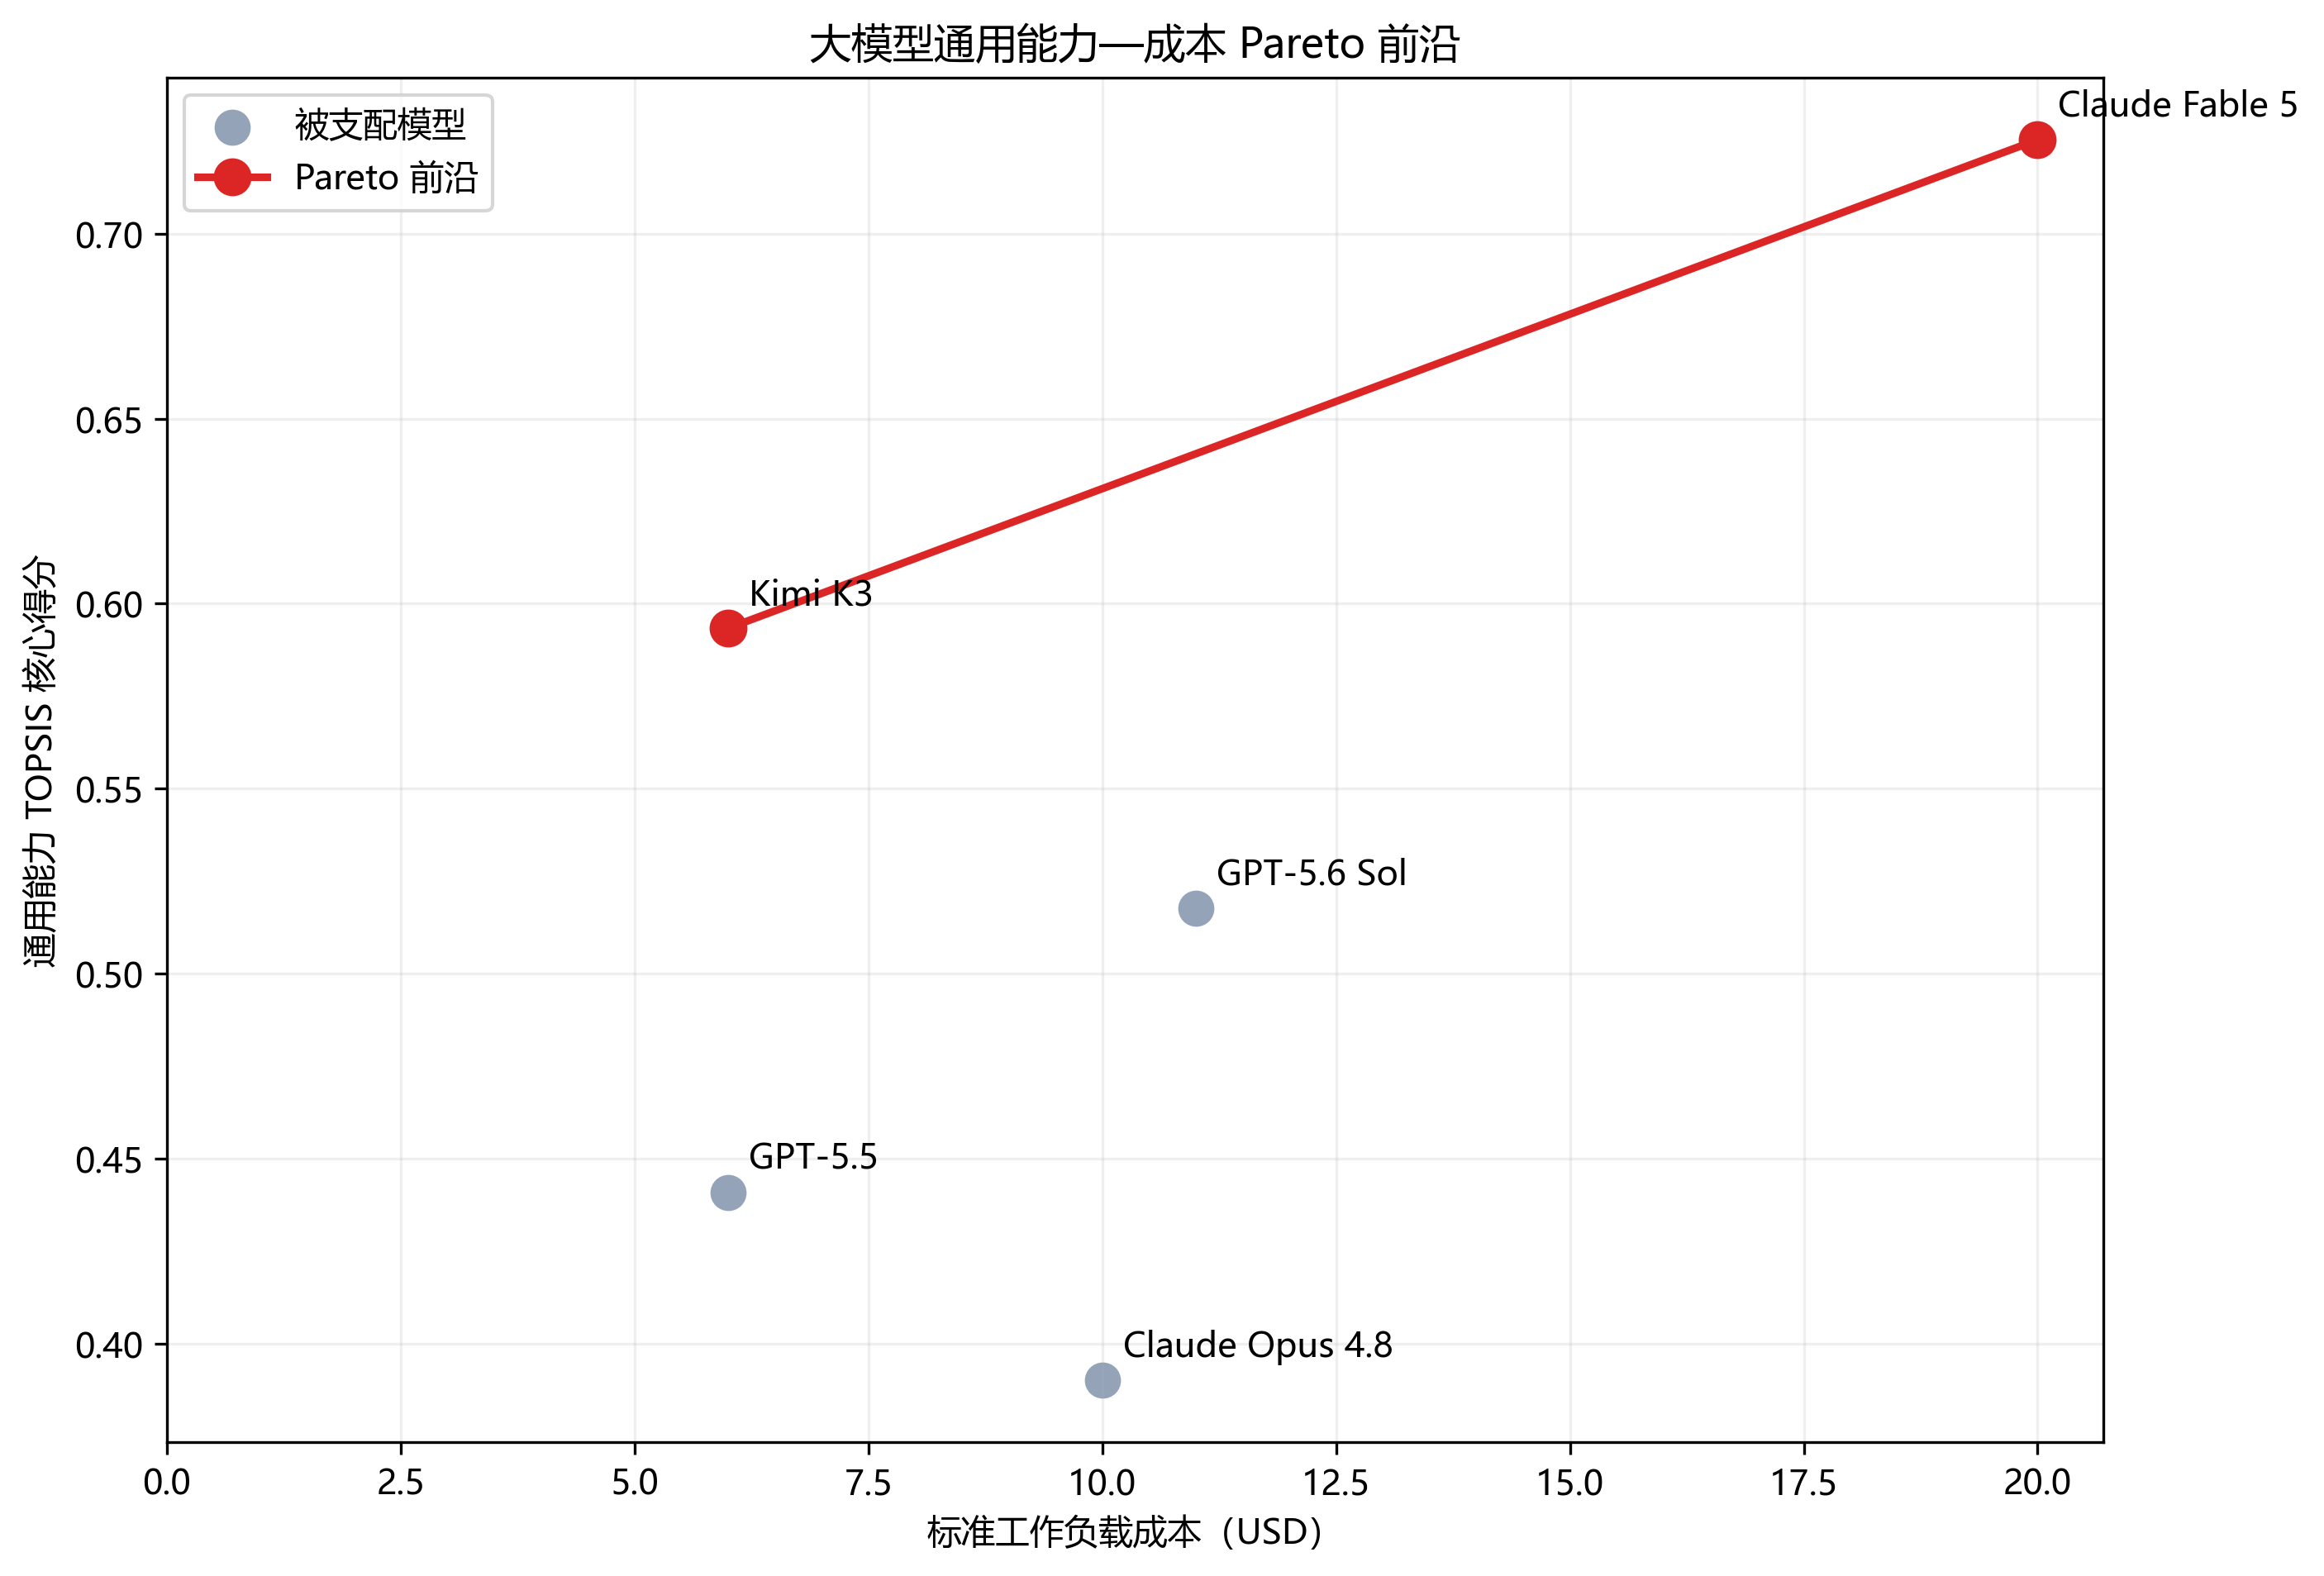
\includegraphics[width=0.86\textwidth]{performance_cost_pareto.png}
  \caption{性能--成本 Pareto 前沿}
  \label{fig:pareto}
\end{figure}

\begin{table}[H]
  \centering
  \caption{预算约束下的模型推荐}
  \label{tab:budget}
  \begin{tabular}{cccc}
    \toprule
    预算/美元 & 可行排名模型数 & 推荐模型 & 推荐模型成本/美元 \\
    \midrule
    6 & 2 & Kimi K3 & 6 \\
    10 & 3 & Kimi K3 & 6 \\
    12 & 4 & Kimi K3 & 6 \\
    16 & 4 & Kimi K3 & 6 \\
    20 & 5 & Claude Fable 5 & 20 \\
    \bottomrule
  \end{tabular}
\end{table}

\subsection{算力能耗数据边界}

赛题要求考察算力消耗，因此本文对公开能耗数据进行了专门可得性审计。严格横向比较需要统一硬件平台、模型精度、batch size、输入与输出长度、reasoning configuration 及 provider 部署条件；但当前公开资料不含满足这些条件的统一模型级 J/token 或 kWh/任务观测，部分闭源 API 亦未披露底层 GPU 与量化精度。因此，本文不用参数量、GPU TDP、推理时延或 API 价格人为推算单次能耗，而将公开 API 货币成本与严格可比的工程效率指标分层分析。算力能耗很重要，但当前只作为无法统一量化的数据边界，不参与正式排名。

为明确能耗在落地决策中的理论位置，定义部署成本框架
\begin{equation}
  C_i^{\mathrm{deploy}}=M_i+c_eE_i,
  \label{eq:deployment-cost}
\end{equation}
其中，$M_i$ 为标准 token 工作负载下的 API 货币成本，$E_i$ 为同一硬件、精度、batch、输入输出长度、reasoning configuration 和 provider 条件下的推理能耗，$c_e$ 为单位能耗折算成本。当前 $M_i$ 有公开可比观测，而 $E_i$ 对候选模型缺乏统一公开观测，故正式实证仅对 $M_i$ 定量，$E_i$ 保留在理论框架中但不代入伪造数值。本文也不以 GPU TDP$\times$时延、参数量$\times$时间、FLOPs、TTFT、E2E 或 API 价格充当 $E_i$ 的代理，因为这些量不等价于实际电力能耗，且闭源 API 的 GPU 型号、数量、量化精度、batch 与并行策略无法统一确认。因此，该框架属于受公开数据约束的分层部署成本模型。

\subsection{严格可比部署效率子分析}

Artificial Analysis 效率数据\cite{aa}的检索日期为 2026 年 8 月 16 日，测量窗口为过去 72 小时滚动窗口，统计量为 P50，故没有唯一的单日测量日期，\texttt{measurement\_date=NA}。TTFT 表示 Time to First Token；Output Speed 单位为 tokens/s；E2E 表示 Artificial Analysis 标准化 500-token 端到端响应时间，不是任意长度回答的总响应时间。

最终 6 个模型中，只有 Kimi K3、GPT-5.6 Sol、Claude Opus 4.8 和 GPT-5.5 同时满足版本、配置、provider 与 workload 一致性要求。Claude Fable 5 的页面配置包含 Opus fallback；GLM-5.2 为 Together AI 第三方部署且量化/精度披露不足，二者均为 \texttt{compatible=false}，原始观测只作补充记录，不参与严格部署效率排名。

\begin{table}[H]
  \centering
  \caption{严格可比效率数据及部署得分}
  \label{tab:efficiency}
  \begin{tabularx}{\textwidth}{L{3.2cm}C{1.6cm}C{2.3cm}C{1.6cm}C{1.9cm}X}
    \toprule
    模型 & TTFT/s & \shortstack{Output Speed\\tokens/s} & E2E/s & 工程效率 & 部署得分 \\
    \midrule
    Kimi K3 & 3.4631 & 39.4660 & 66.8087 & 0.5695 & 0.5862 \\
    GPT-5.6 Sol & 142.4287 & 73.7378 & 149.2095 & 0.2283 & 0.4309 \\
    Claude Opus 4.8 & 24.7382 & 61.0633 & 32.9264 & 0.7595 & 0.5010 \\
    GPT-5.5 & 48.4270 & 89.5060 & 54.0132 & 0.8317 & 0.5582 \\
    \bottomrule
  \end{tabularx}
\end{table}

工程效率由 TTFT 成本型正向化、输出速度效益型正向化和 E2E 成本型正向化后等权平均；部署得分由 70\% 通用能力核心得分与 30\% 工程效率组成。该结论只覆盖表~\ref{tab:efficiency}中的 4 个模型，不能扩展为 6 模型效率排名。

图~\ref{fig:engineering-efficiency} 展示严格可比的 4 个模型的三项效率构成、工程效率与部署得分。
\begin{figure}[htbp]
  \centering
  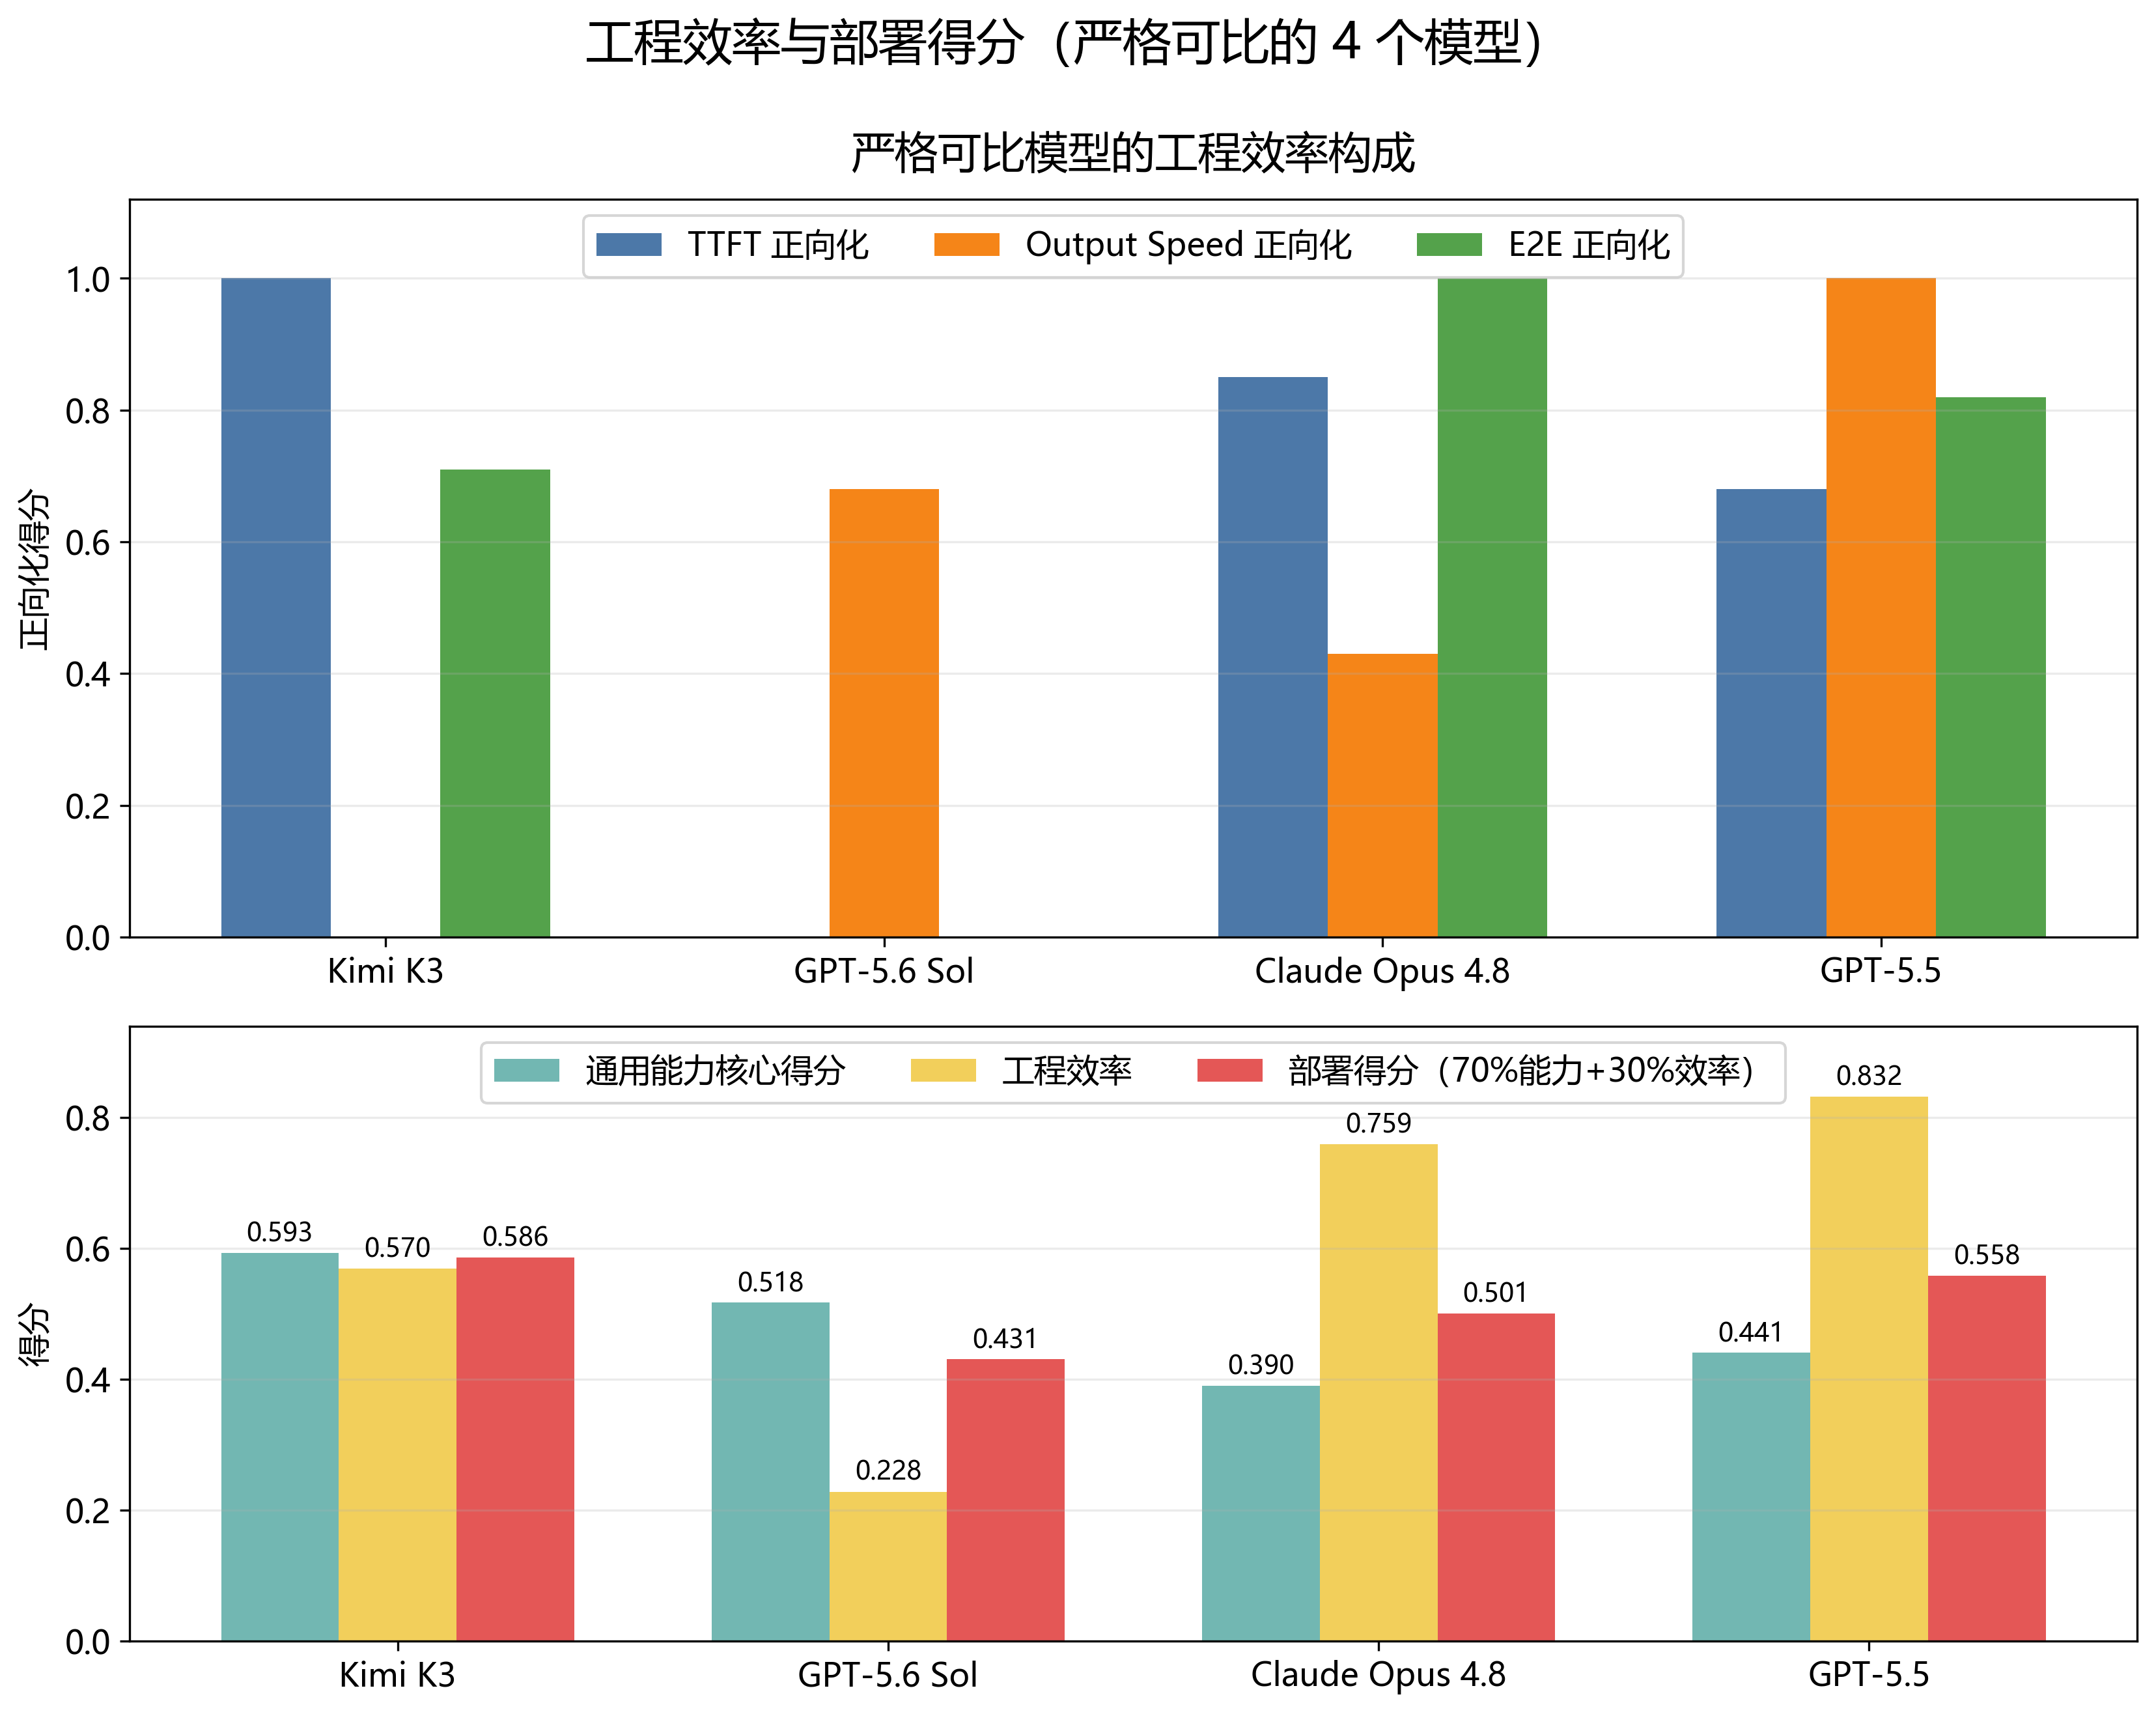
\includegraphics[width=0.84\textwidth]{engineering_efficiency_enhanced.png}
  \caption{严格可比模型的工程效率与部署得分}
  \label{fig:engineering-efficiency}
\end{figure}

\subsection{成本--性能探索性关系}

对 5 个具有完整通用能力排名的模型拟合，其中 $\mathrm{Performance}$ 表示问题一的通用能力核心得分：
\begin{equation}
  \mathrm{Performance}=0.199408+0.148104\ln(\mathrm{Cost}),
  \label{eq:regression}
\end{equation}
得到 $R^2=0.314672$、调整 $R^2=0.086230$、$\mathrm{RMSE}=0.097773$。由于 $n=5$ 且解释力有限，式~\eqref{eq:regression}只描述当前样本内的探索性弱正相关，不构成成本与性能之间的普遍定律或因果证据。

五个完整模型的观测点与对数拟合曲线如图~\ref{fig:cost-regression} 所示。
\begin{figure}[htbp]
  \centering
  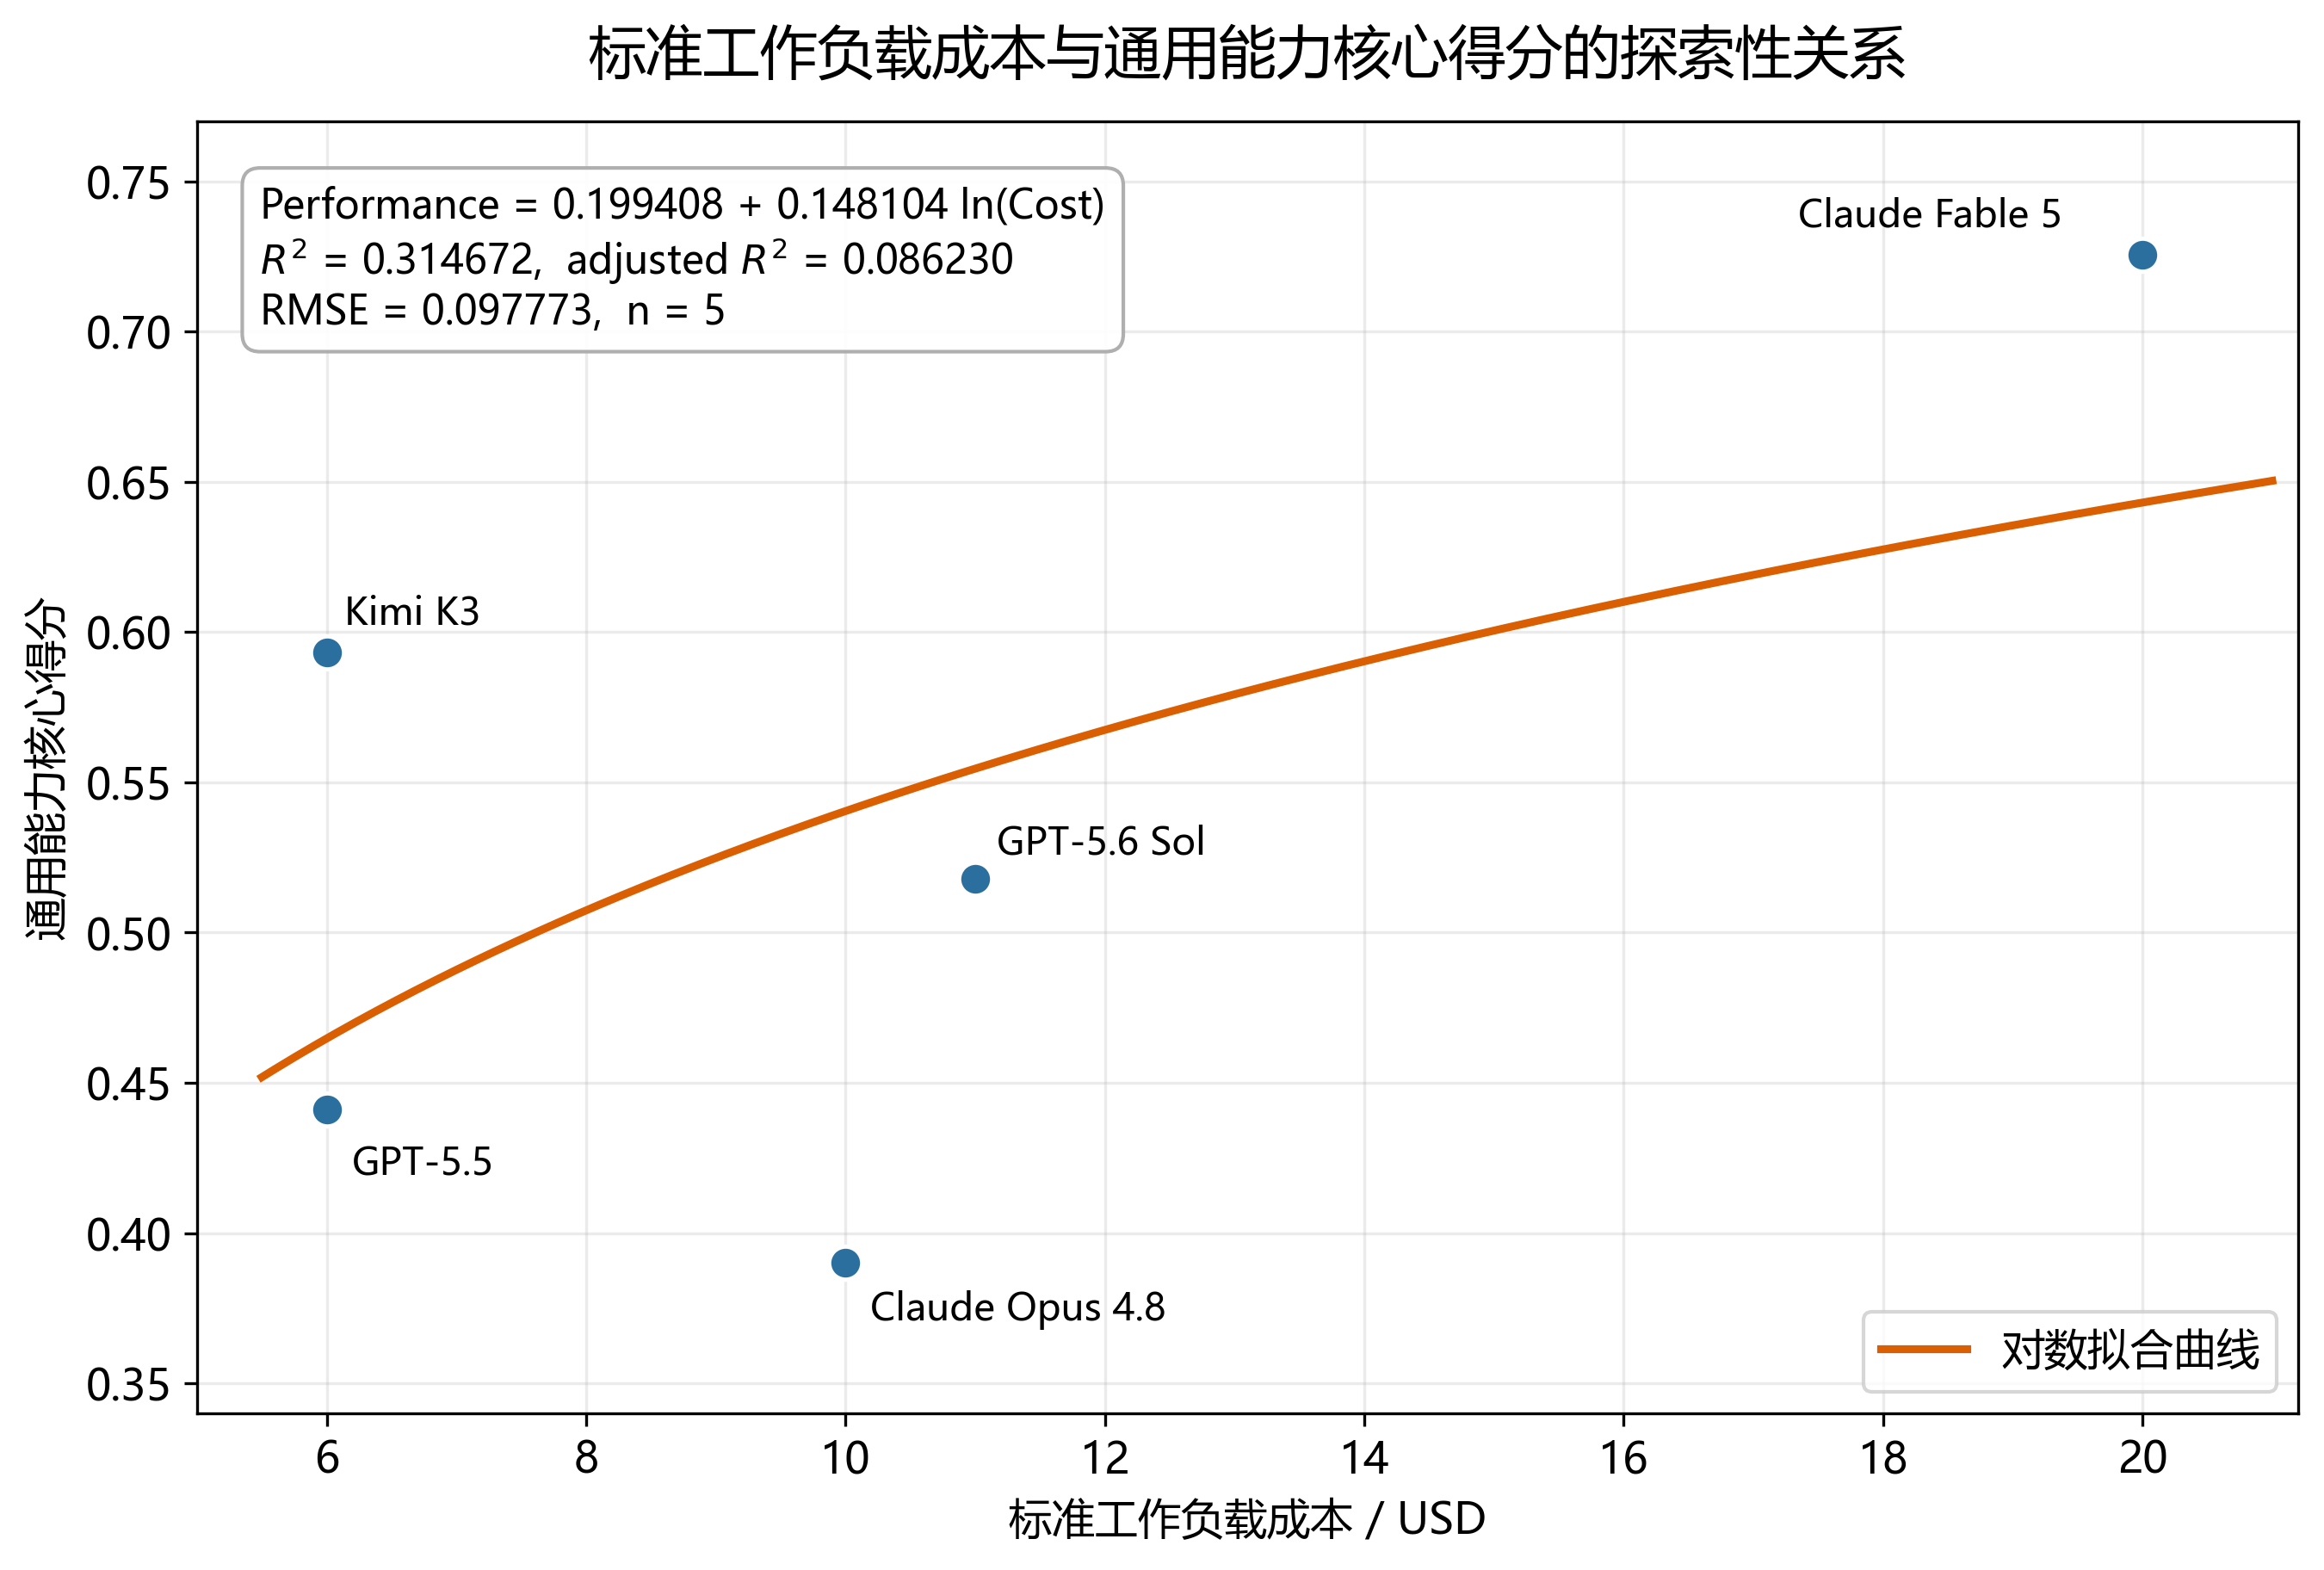
\includegraphics[width=0.82\textwidth]{cost_regression_enhanced.png}
  \caption{标准工作负载成本与通用能力核心得分的探索性关系}
  \label{fig:cost-regression}
\end{figure}

\section{稳健性分析}

\subsection{方法与参数稳健性}

方法稳健性方面，以熵权法替代 CRITIC 计算权重，5 个完整模型的排名与 CRITIC--TOPSIS 完全一致。参数稳健性方面，对 9 个 CRITIC 权重分别乘以 0.8、0.9、1.1 和 1.2，每次重新归一化并重算 TOPSIS，共形成 36 个确定性单因素扰动场景。

所有扰动中 Claude Fable 5、Kimi K3 与 GPT-5.6 Sol 始终保持第 1、2、3 名。只有 HLE-Full 权重乘以 1.2 时，Claude Opus 4.8 与 GPT-5.5 交换第 4、5 名；扰动排名相对基准的最低 Kendall $\tau$ 为 0.8。因此，前三结论在当前局部扰动范围内稳定，但这 36 次检验不能替代全局不确定性分析。

36 组单因素权重扰动下的 Kendall $\tau$ 如图~\ref{fig:perturbation} 所示。
\begin{figure}[htbp]
  \centering
  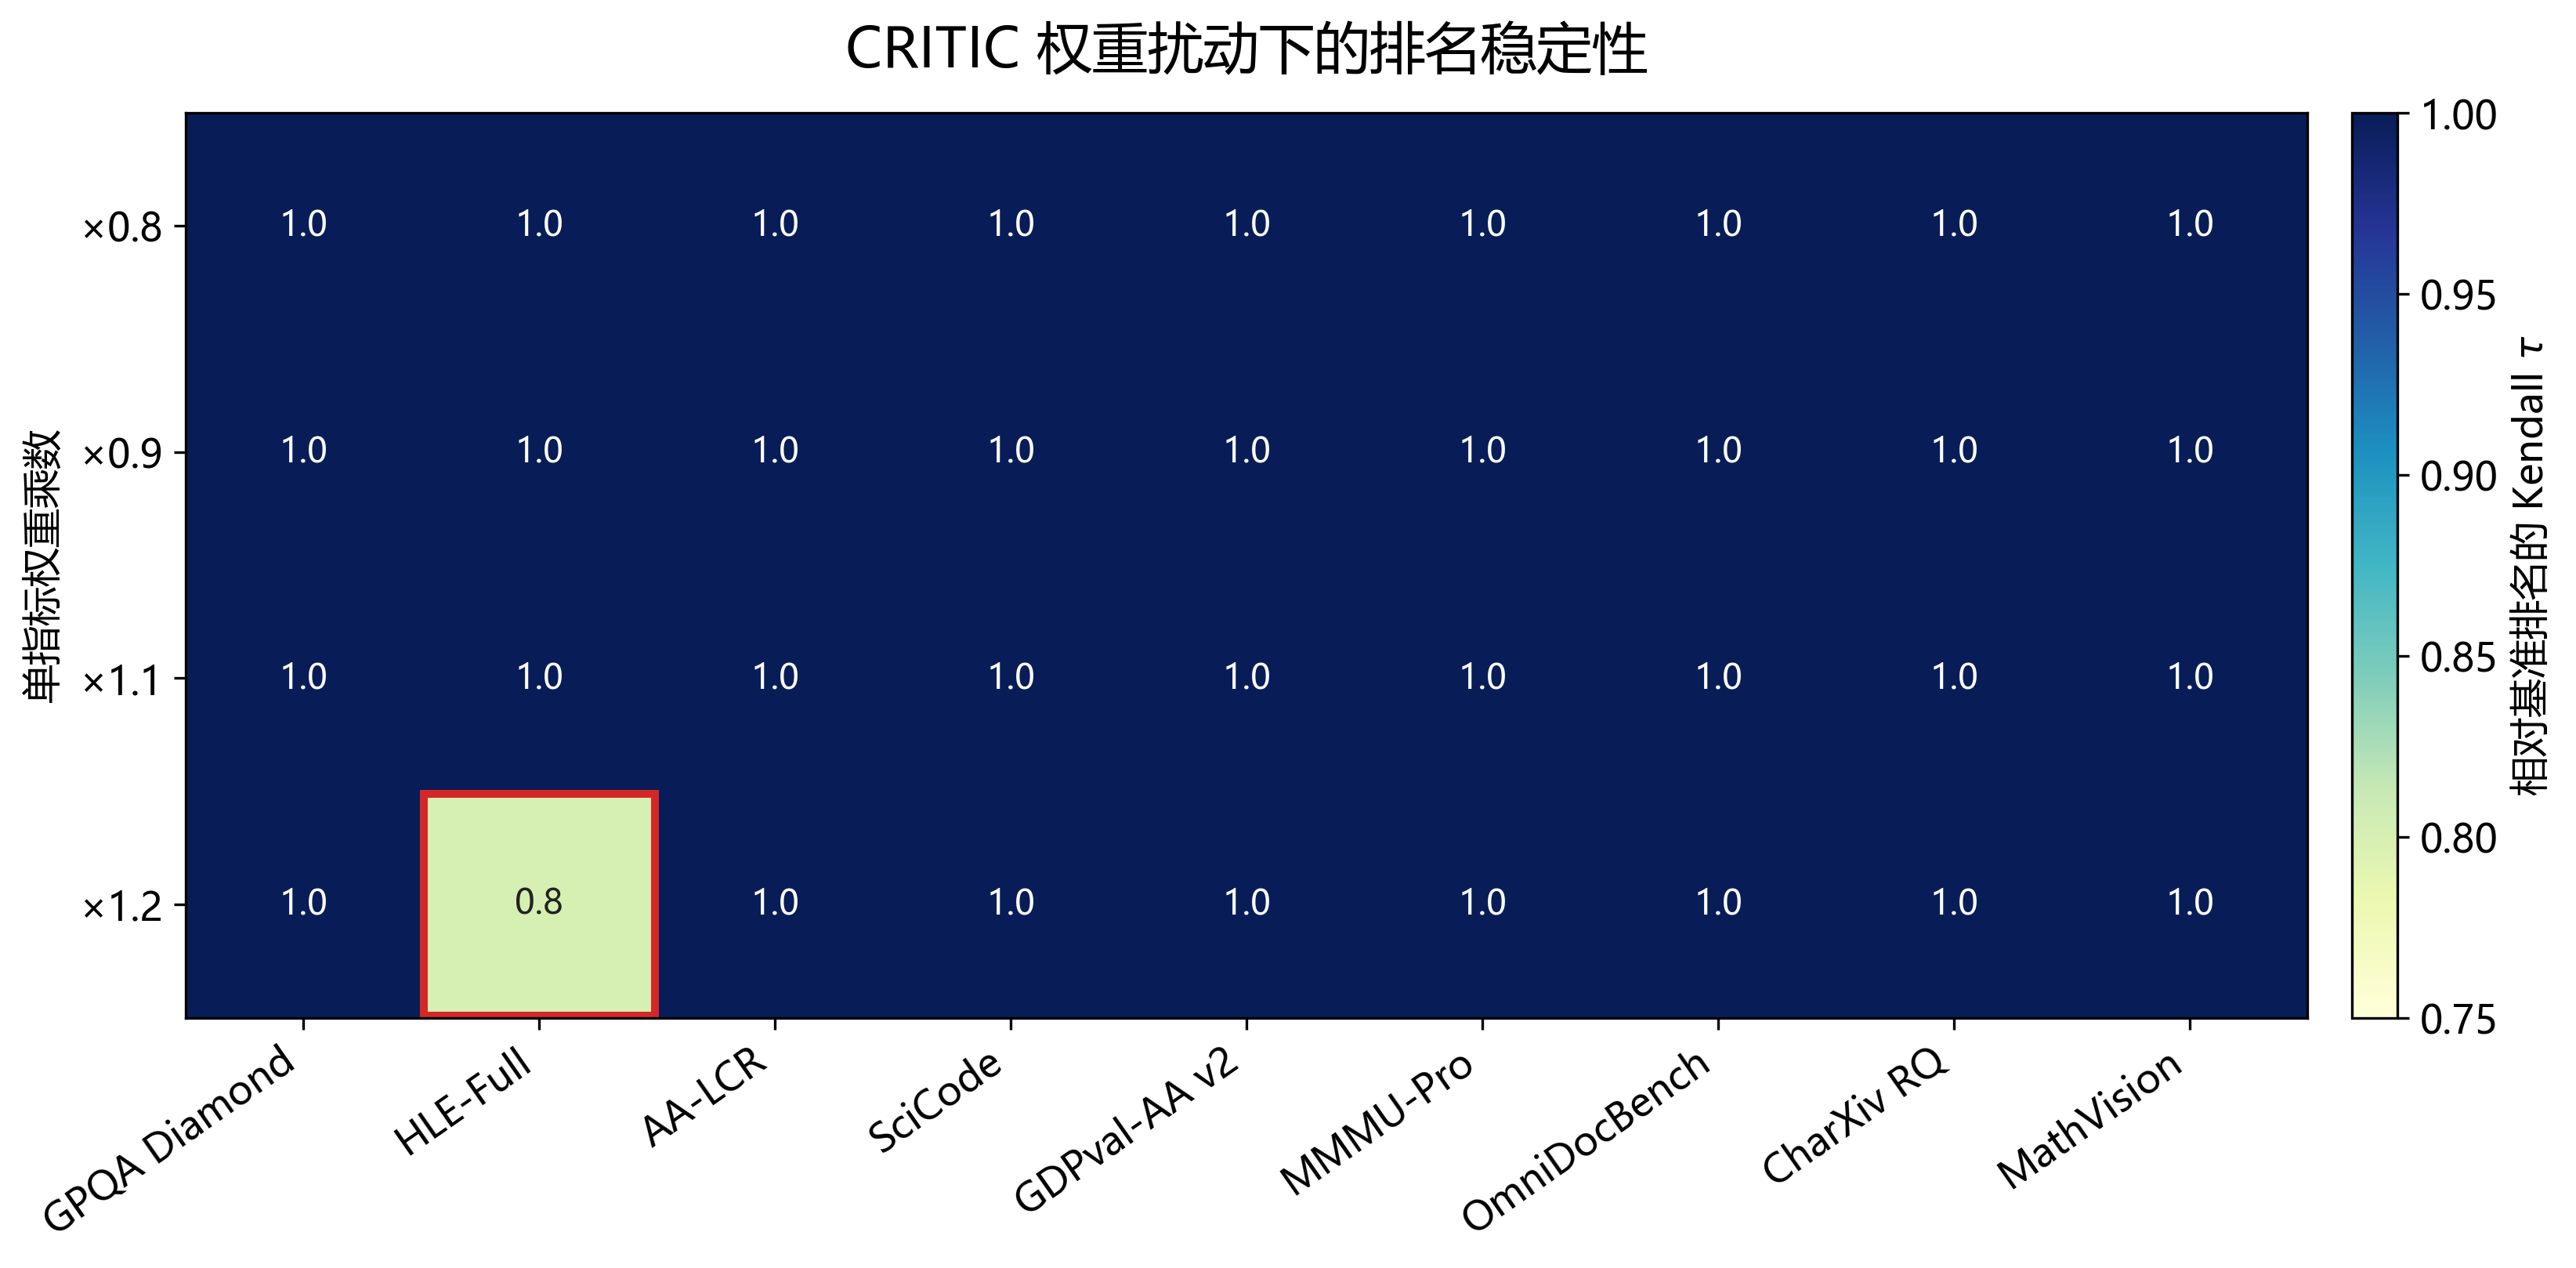
\includegraphics[width=0.88\textwidth]{perturbation_robustness_enhanced.png}
  \caption{CRITIC 权重扰动下的排名稳定性}
  \label{fig:perturbation}
\end{figure}

\begin{table}[H]
  \centering
  \caption{权重扰动下的排名稳定性}
  \label{tab:stability}
  \begin{tabular}{lccccc}
    \toprule
    模型 & 基准排名 & 最低排名 & 最高排名 & 平均排名 & 第一频率 \\
    \midrule
    Claude Fable 5 & 1 & 1 & 1 & 1.0000 & 1.0000 \\
    Kimi K3 & 2 & 2 & 2 & 2.0000 & 0 \\
    GPT-5.6 Sol & 3 & 3 & 3 & 3.0000 & 0 \\
    GPT-5.5 & 4 & 4 & 5 & 4.0278 & 0 \\
    Claude Opus 4.8 & 5 & 4 & 5 & 4.9722 & 0 \\
    \bottomrule
  \end{tabular}
\end{table}

\subsection{样本集合敏感性检验}

正式 CRITIC 对各指标使用其可得的 5 或 6 个模型计算总体标准差，并以逐对完整观测计算 Pearson 相关；主 TOPSIS 则只对 9 项指标均完整的 5 个模型排序。为检验缺失模式及样本集合对客观权重的影响，进一步排除 GLM-5.2 的部分观测，以与主 TOPSIS 完全相同的 Claude Fable 5、Kimi K3、GPT-5.6 Sol、GPT-5.5 和 Claude Opus 4.8 构成 $5\times9$ 完整矩阵。在标准化方法、总体标准差、Pearson 相关、CRITIC 冲突度和 TOPSIS 算法均保持不变的条件下，仅将 CRITIC 的计算样本固定为这 5 个模型并重新进行对照计算。

对照权重相对正式权重的最大绝对变化为 0.00905，平均绝对变化为 0.00364；HLE-Full、OmniDocBench 和 AA-LCR 仍依次为权重前三，只有低权重指标的内部次序发生小幅变化。5 个模型的完整综合排名保持不变，正式排名与对照排名的 Spearman 系数和 Kendall $\tau$ 均为 1。Kimi K3 在两种口径下均排名第 2，与第 1 名的 TOPSIS 分差由 0.1320 缩小至 0.1210。该结果表明，主排名对当前样本缺失处理具有较强的局部稳健性，但该对照只作为样本敏感性证据，不替换正式 CRITIC 权重或正式 TOPSIS 结果。

\subsection{场景组合系数敏感性}

为检验客观信息与场景偏好组合比例对问题二结论的影响，在不改变 CRITIC 权重、人工偏好向量及 TOPSIS 算法的条件下，取 $\lambda=0.3,0.4,0.5,0.6,0.7$ 进行合理邻域敏感性分析。这里 $\lambda$ 越大表示 CRITIC 客观权重影响增强、场景人工偏好影响减弱；该离散网格不代表全部可能偏好，也不用于证明 $\lambda=0.5$ 最优。

科研长文本场景中，Kimi K3 相对 Claude Fable 5 的得分差随 $\lambda$ 增大由 0.063106 持续缩小，在 $\lambda=0.5$ 时为 0.007590，在 $\lambda=0.6$ 时变为 $-0.020700$。因此，在所检验的离散网格上，榜首切换区间只能确定为 $[0.5,0.6]$，不能据此给出精确临界值。Kimi K3 的基准第一具有条件性，其优势部分来自科研场景对长文本与科研文档能力的定向加权；但前三模型集合始终不变，GPT-5.6 Sol、GPT-5.5 与 Claude Opus 4.8 分别始终处于第 3、4、5 位，最低 Spearman 系数为 0.9、最低 Kendall $\tau$ 为 0.8，说明整体模型梯队仍具有较高稳定性。

大众日常对话和代码开发场景在 $\lambda=0.3$--$0.7$ 内完整排名均保持不变，最低 Spearman 与 Kendall $\tau$ 均为 1。Claude Fable 5 对 Kimi K3 的领先差在日常对话中由 0.068175 扩大至 0.105107，在代码开发中由 0.071038 扩大至 0.106507。三类场景的汇总结论见表~\ref{tab:lambda-sensitivity}。

\begin{table}[H]
  \centering
  \caption{场景组合系数的局部敏感性汇总}
  \label{tab:lambda-sensitivity}
  \begin{tabularx}{\textwidth}{L{2.2cm}C{1.5cm}L{3.2cm}C{1.5cm}C{1.5cm}C{1.5cm}X}
    \toprule
    场景 & $\lambda$ 范围 & 榜首稳定性 & 前三集合 & 最低 Spearman & 最低 Kendall & 结论 \\
    \midrule
    科研长文本 & 0.3--0.7 & Kimi/Fable 切换 & 稳定 & 0.9 & 0.8 & 对 $\lambda$ 中度敏感 \\
    大众日常对话 & 0.3--0.7 & Fable 始终第一 & 稳定 & 1.0 & 1.0 & 高度稳定 \\
    代码开发 & 0.3--0.7 & Fable 始终第一 & 稳定 & 1.0 & 1.0 & 高度稳定 \\
    \bottomrule
  \end{tabularx}
\end{table}

\section{模型评价与局限}

\subsection{方法特点}

本文从原始来源、精确版本和评测设置开始建立可追溯链路，缺失值处理保守；CRITIC 权重、TOPSIS 排名、场景权重、货币成本和稳健性结果均可由冻结脚本复算。能力、货币成本和效率采用分层分析，避免把价格或时延在通用能力核心得分中重复计权。

\subsection{局限性}

\begin{enumerate}[label=(\arabic*),leftmargin=3em]
  \item 核心 Benchmark cohort 高度集中于厂商技术报告的统一对照数据，尽管设置统一且可追溯，仍可能存在厂商报告偏差。
  \item 部分新模型接近截止日才发布，导致严格可比分项覆盖不足；最终池筛选不能解释为单纯追求覆盖率。
  \item 相关性、CRITIC 和回归只基于 5--6 个模型，统计量容易随样本池改变，不宜外推。0.85 相关阈值仅是冗余复核规则，相关分析不进行总体显著性推断；尽管完整样本对照未改变排名，这仍只是当前小样本模型池内的稳健性证据，不能外推至任意模型集合。
  \item 严格部署效率只覆盖 6 个最终模型中的 4 个；Fable 与 GLM 的不兼容观测不能用于横向效率高低判断。
  \item Artificial Analysis 指标是过去 72 小时滚动 P50，只代表 2026 年 8 月 16 日检索时段附近的 provider 表现。
  \item API 成本只对应 100 万输入加 20 万输出 token 的固定 workload 与截面标准价，未完整建模缓存、Batch、长上下文阶梯价、区域加价和峰谷套餐。
  \item 算力能耗缺乏统一硬件、精度、批量和推理设置下的公开可比观测，故未进行人工估算或能耗排名。
  \item 三类场景的人工偏好为题意驱动设定，尚未经过真实专家问卷或团队成对比较校准。
  \item 当前核心能力层未将知识事实准确性单列为独立评价指标；受版本、测试设置及公开数据同口径可比性约束，本文未将异源事实性 Benchmark 强行并入冻结核心矩阵。后续若获得同版本、同设置且覆盖充分的公开事实性基准，可进一步补充该维度。
  \item 36 次扰动是局部单因素敏感性分析，不能代替全局不确定性传播或大规模随机模拟。
\end{enumerate}

\subsection{改进方向}

未来可建立滚动数据更新与版本、价格时间戳管理机制，并在覆盖充分后扩展模型池及知识事实准确性指标；使用真实专家调查、Delphi 法或 AHP 校准场景偏好；在统一 GPU、精度、batch 和推理设置下实测 J/token 等能耗；进一步将静态单模型选型扩展为预算、时延与质量多约束下的动态模型路由。

\section{结论与建议}

在不插补缺失数据的前提下，Claude Fable 5、Kimi K3 与 GPT-5.6 Sol 获得通用能力综合评价前三。本文的综合评价采用分层框架：通用能力由九项 Benchmark 形成核心得分，工程效率、货币成本和能耗边界在落地决策层进一步分析。Kimi K3 的竞争力集中在长文本、文档理解和科研材料处理，HLE-Full 所代表的极高难开放推理是其主要短板。在等比例组合的基准设定下，科研长文本场景 Kimi K3 排名第一；但组合系数敏感性表明，其与 Claude Fable 5 的榜首位置具有条件性，科研场景选型应结合决策者对客观通用能力与场景专门需求的侧重程度。日常对话与代码开发场景下 Claude Fable 5 保持第一。跨场景差异本质上来自模型能力画像与场景权重结构的匹配程度不同，并通过加权空间中的正、负理想解距离反映在 TOPSIS 排名中。

在当前标准 API 工作负载下，Kimi K3 与 Claude Fable 5 构成性能--成本 Pareto 前沿。在本文考察的 6、10、12 和 16 美元预算点下均推荐 Kimi K3；预算达到 20 美元且追求最高通用能力时推荐 Claude Fable 5。部署效率结论只适用于 4 个严格 compatible 模型。理论部署成本模型包含能耗项，但由于统一能耗观测不可得，本文不对其进行伪精确估算。熵权对照和权重扰动支持前三名的局部稳定性，但所有结论均应限定在数据截面、固定 cohort 和小样本范围内。

\section{AI 工具使用声明}

本参赛队在竞赛过程中使用了 ChatGPT 与 Codex 辅助代码调试、数据核验、论文结构检查、格式规范核验、可视化检查及语言表述优化\cite{chatgpt-ai,codex-ai}。核心建模方案、指标筛选原则、正式数据选择、数学计算、结果解释和最终结论均由参赛队员审阅并确认。具体 AI 使用环节、关键交互及人工修改情况见支撑材料《人工智能工具使用详情》；论文结构检查和部分语言表述使用了 AI 辅助优化。

\begin{thebibliography}{99}
  \small
  \setlength{\itemsep}{1pt}
  \setlength{\parskip}{0pt}
  \bibitem{kimi-k3}
  Moonshot AI. Kimi K3 Technical Report[EB/OL].
  \url{https://github.com/MoonshotAI/Kimi-K3}, 2026-07-16.

  \bibitem{aa}
  Artificial Analysis. AI Model and API Provider Performance Benchmarking[EB/OL].
  \url{https://artificialanalysis.ai/}, accessed 2026-08-16.

  \bibitem{kimi-blog}
  Moonshot AI. Kimi K3 Official Blog[EB/OL].
  \url{https://www.kimi.com/blog/kimi-k3}, 2026-07-16, accessed 2026-08-16.

  \bibitem{openai-launch}
  OpenAI. GPT-5.6 Launch Report[EB/OL].
  \url{https://openai.com/index/gpt-5-6/}, accessed 2026-08-16.

  \bibitem{openai-models}
  OpenAI. API Model Comparison[EB/OL].
  \url{https://developers.openai.com/api/docs/models/compare/}, accessed 2026-08-16.

  \bibitem{openai-pricing}
  OpenAI. API Pricing[EB/OL].
  \url{https://platform.openai.com/docs/pricing/}, accessed 2026-08-16.

  \bibitem{anthropic-models}
  Anthropic. Claude Models Overview[EB/OL].
  \url{https://platform.claude.com/docs/zh-CN/about-claude/models}, accessed 2026-08-16.

  \bibitem{anthropic-pricing}
  Anthropic. Claude API Pricing[EB/OL].
  \url{https://platform.claude.com/docs/en/about-claude/pricing}, accessed 2026-08-17.

  \bibitem{zai-launch}
  Z.ai. GLM-5.2 Official Launch Report[EB/OL].
  \url{https://z.ai/blog/glm-5.2}, 2026-06-16, accessed 2026-08-17.

  \bibitem{zhipu-pricing}
  Zhipu AI. GLM API Pricing[EB/OL].
  \url{https://open.bigmodel.cn/pricing}, accessed 2026-08-16.

  \bibitem{topsis}
  Hwang C L, Yoon K. Multiple Attribute Decision Making: Methods and Applications[M].
  Berlin: Springer-Verlag, 1981.

  \bibitem{critic}
  Diakoulaki D, Mavrotas G, Papayannakis L. Determining objective weights in multiple criteria problems: The CRITIC method[J]. Computers \& Operations Research, 1995, 22(7): 763--770. DOI: 10.1016/0305-0548(94)00059-H.

  \bibitem{chatgpt-ai}
  ChatGPT，GPT-5.6 Sol，OpenAI，2026-08-16--2026-08-19.

  \bibitem{codex-ai}
  Codex，GPT-5.6 Sol，OpenAI，2026-08-16--2026-08-19.
\end{thebibliography}

\clearpage
\appendix
\section{支撑材料文件清单}
\begingroup\small
\begin{longtable}{C{0.9cm}L{9.2cm}L{4.3cm}}
\toprule
序号 & 相对路径 & 文件说明 \\
\midrule
\endfirsthead
\toprule
序号 & 相对路径 & 文件说明 \\
\midrule
\endhead
1 & \path{AI_CHATGPT_RECORDS_NEED_USER.txt} & 待用户补充的真实 ChatGPT 交互说明 \\
2 & \path{data/merged/.gitkeep} & 模型合并数据 \\
3 & \path{data/merged/model_dataset.csv} & 模型合并数据 \\
4 & \path{data/model_candidates.csv} & 模型池或数据配置 \\
5 & \path{data/processed/.gitkeep} & 模型使用的处理后数据 \\
6 & \path{data/processed/core_benchmark_long.csv} & 模型使用的处理后数据 \\
7 & \path{data/processed/core_benchmark_matrix.csv} & 模型使用的处理后数据 \\
8 & \path{data/processed/indicator_quality.csv} & 模型使用的处理后数据 \\
9 & \path{data/processed/model_attributes.csv} & 模型使用的处理后数据 \\
10 & \path{data/processed/phase2_quality_report.csv} & 模型使用的处理后数据 \\
11 & \path{data/raw/benchmark_scores.csv} & 冻结原始数据 \\
12 & \path{data/raw/cost_efficiency.csv} & 冻结原始数据 \\
13 & \path{data/raw/model_metadata.csv} & 冻结原始数据 \\
14 & \path{data/sources/benchmark_sources.csv} & 公开数据来源索引 \\
15 & \path{data/sources/efficiency_sources.csv} & 公开数据来源索引 \\
16 & \path{data/sources/metadata_sources.csv} & 公开数据来源索引 \\
17 & \path{README.txt} & 支撑材料结构、运行环境与复现说明 \\
18 & \path{results/.gitkeep} & 论文模型结果或图表 \\
19 & \path{results/benchmark_coverage.csv} & 论文模型结果或图表 \\
20 & \path{results/core_indicator_selection.csv} & 论文模型结果或图表 \\
21 & \path{results/efficiency_configuration_review.csv} & 论文模型结果或图表 \\
22 & \path{results/efficiency_staging.csv} & 论文模型结果或图表 \\
23 & \path{results/final_model_summary.csv} & 论文模型结果或图表 \\
24 & \path{results/phase3/descriptive_statistics.csv} & 论文模型结果或图表 \\
25 & \path{results/phase3/indicator_screening.csv} & 论文模型结果或图表 \\
26 & \path{results/phase3/pearson_correlation.csv} & 论文模型结果或图表 \\
27 & \path{results/phase3/redundancy_flags.csv} & 论文模型结果或图表 \\
28 & \path{results/phase3/spearman_correlation.csv} & 论文模型结果或图表 \\
29 & \path{results/phase4/critic_weights.csv} & 论文模型结果或图表 \\
30 & \path{results/phase4/general_ranking.csv} & 论文模型结果或图表 \\
31 & \path{results/phase4/kimi_strengths_weaknesses.csv} & 论文模型结果或图表 \\
32 & \path{results/phase4/normalized_scores.csv} & 论文模型结果或图表 \\
33 & \path{results/phase4b/glm_official_hle_note.csv} & 论文模型结果或图表 \\
34 & \path{results/phase4b/glm_partial_comparison.csv} & 论文模型结果或图表 \\
35 & \path{results/phase4b/glm_partial_comparison.png} & 论文模型结果或图表 \\
36 & \path{results/phase5/scenario_rankings.csv} & 论文模型结果或图表 \\
37 & \path{results/phase5/scenario_weights.csv} & 论文模型结果或图表 \\
38 & \path{results/phase6/budget_recommendations.csv} & 论文模型结果或图表 \\
39 & \path{results/phase6/engineering_efficiency.csv} & 论文模型结果或图表 \\
40 & \path{results/phase6/performance_cost.csv} & 论文模型结果或图表 \\
41 & \path{results/phase7/cost_performance_regression.csv} & 论文模型结果或图表 \\
42 & \path{results/phase7/method_comparison.csv} & 论文模型结果或图表 \\
43 & \path{results/phase7/rank_correlation.csv} & 论文模型结果或图表 \\
44 & \path{results/phase7/rank_stability.csv} & 论文模型结果或图表 \\
45 & \path{results/phase7/weight_method_comparison.csv} & 论文模型结果或图表 \\
46 & \path{results/phase7/weight_perturbation_rankings.csv} & 论文模型结果或图表 \\
47 & \path{results/q1/critic_weights.csv} & 论文模型结果或图表 \\
48 & \path{results/q1/critic_weights_bar.png} & 论文模型结果或图表 \\
49 & \path{results/q1/data_quality_report.csv} & 论文模型结果或图表 \\
50 & \path{results/q1/final_indicator_system.csv} & 论文模型结果或图表 \\
51 & \path{results/q1/high_correlation_pairs.csv} & 论文模型结果或图表 \\
52 & \path{results/q1/kimi_k3_gap.png} & 论文模型结果或图表 \\
53 & \path{results/q1/kimi_k3_metric_analysis.csv} & 论文模型结果或图表 \\
54 & \path{results/q1/kimi_k3_radar.png} & 论文模型结果或图表 \\
55 & \path{results/q1/normalized_data.csv} & 论文模型结果或图表 \\
56 & \path{results/q1/pearson_correlation.csv} & 论文模型结果或图表 \\
57 & \path{results/q1/pearson_heatmap.png} & 论文模型结果或图表 \\
58 & \path{results/q1/rank_stability.csv} & 论文模型结果或图表 \\
59 & \path{results/q1/removed_metrics.csv} & 论文模型结果或图表 \\
60 & \path{results/q1/selected_metrics.csv} & 论文模型结果或图表 \\
61 & \path{results/q1/sensitivity_analysis.csv} & 论文模型结果或图表 \\
62 & \path{results/q1/spearman_correlation.csv} & 论文模型结果或图表 \\
63 & \path{results/q1/spearman_heatmap.png} & 论文模型结果或图表 \\
64 & \path{results/q1/topsis_ranking.csv} & 论文模型结果或图表 \\
65 & \path{results/q1/topsis_ranking_bar.png} & 论文模型结果或图表 \\
66 & \path{results/q2/coding_ranking.csv} & 论文模型结果或图表 \\
67 & \path{results/q2/dialogue_ranking.csv} & 论文模型结果或图表 \\
68 & \path{results/q2/kimi_k3_scenario_analysis.csv} & 论文模型结果或图表 \\
69 & \path{results/q2/kimi_k3_scenario_radar.png} & 论文模型结果或图表 \\
70 & \path{results/q2/rank_change.png} & 论文模型结果或图表 \\
71 & \path{results/q2/rank_change_analysis.csv} & 论文模型结果或图表 \\
72 & \path{results/q2/research_ranking.csv} & 论文模型结果或图表 \\
73 & \path{results/q2/scenario_rank_comparison.png} & 论文模型结果或图表 \\
74 & \path{results/q2/scenario_rankings.csv} & 论文模型结果或图表 \\
75 & \path{results/q2/scenario_score_heatmap.png} & 论文模型结果或图表 \\
76 & \path{results/q2/scenario_sensitivity.csv} & 论文模型结果或图表 \\
77 & \path{results/q2/scenario_stability.csv} & 论文模型结果或图表 \\
78 & \path{results/q2/scenario_weights.csv} & 论文模型结果或图表 \\
79 & \path{results/q2/scenario_weights_heatmap.png} & 论文模型结果或图表 \\
80 & \path{results/q3/budget_selection.csv} & 论文模型结果或图表 \\
81 & \path{results/q3/budget_selection.png} & 论文模型结果或图表 \\
82 & \path{results/q3/cost_data_audit.csv} & 论文模型结果或图表 \\
83 & \path{results/q3/deploy_scores.csv} & 论文模型结果或图表 \\
84 & \path{results/q3/engineering_efficiency.png} & 论文模型结果或图表 \\
85 & \path{results/q3/kimi_k3_cost_analysis.csv} & 论文模型结果或图表 \\
86 & \path{results/q3/pareto_analysis.csv} & 论文模型结果或图表 \\
87 & \path{results/q3/performance_cost.csv} & 论文模型结果或图表 \\
88 & \path{results/q3/performance_cost_fit.png} & 论文模型结果或图表 \\
89 & \path{results/q3/performance_cost_pareto.png} & 论文模型结果或图表 \\
90 & \path{results/q3/performance_cost_regression.csv} & 论文模型结果或图表 \\
91 & \path{results/q3/sensitivity_analysis.csv} & 论文模型结果或图表 \\
92 & \path{source/figures/critic_weights.svg} & 模型计算、验证或可视化源文件 \\
93 & \path{source/figures/general_ranking.svg} & 模型计算、验证或可视化源文件 \\
94 & \path{source/figures/performance_cost_pareto.svg} & 模型计算、验证或可视化源文件 \\
95 & \path{source/figures/scenario_rank_changes.svg} & 模型计算、验证或可视化源文件 \\
96 & \path{source/requirements.txt} & 模型计算、验证或可视化源文件 \\
97 & \path{source/run_all.ps1} & 模型计算、验证或可视化源文件 \\
98 & \path{source/scripts/analyze_phase3_indicators.py} & 模型计算、验证或可视化源文件 \\
99 & \path{source/scripts/analyze_phase7_robustness.py} & 模型计算、验证或可视化源文件 \\
100 & \path{source/scripts/artificial_analysis_targets.json} & 模型计算、验证或可视化源文件 \\
101 & \path{source/scripts/build_member_b_data.py} & 模型计算、验证或可视化源文件 \\
102 & \path{source/scripts/build_paper.py} & 模型计算、验证或可视化源文件 \\
103 & \path{source/scripts/check_coverage.py} & 模型计算、验证或可视化源文件 \\
104 & \path{source/scripts/fetch_artificial_analysis_efficiency.py} & 模型计算、验证或可视化源文件 \\
105 & \path{source/scripts/generate_figures.py} & 模型计算、验证或可视化源文件 \\
106 & \path{source/scripts/merge_data.py} & 模型计算、验证或可视化源文件 \\
107 & \path{source/scripts/model_phase4_critic_topsis.py} & 模型计算、验证或可视化源文件 \\
108 & \path{source/scripts/model_phase5_scenarios.py} & 模型计算、验证或可视化源文件 \\
109 & \path{source/scripts/model_phase6_cost_benefit.py} & 模型计算、验证或可视化源文件 \\
110 & \path{source/scripts/phase2_core_cohorts.csv} & 模型计算、验证或可视化源文件 \\
111 & \path{source/scripts/phase5_scenario_priorities.csv} & 模型计算、验证或可视化源文件 \\
112 & \path{source/scripts/process_phase2_data.py} & 模型计算、验证或可视化源文件 \\
113 & \path{source/scripts/run_glm_supplement.py} & 模型计算、验证或可视化源文件 \\
114 & \path{source/scripts/run_pipeline.py} & 模型计算、验证或可视化源文件 \\
115 & \path{source/scripts/run_q1.py} & 模型计算、验证或可视化源文件 \\
116 & \path{source/scripts/run_q2.py} & 模型计算、验证或可视化源文件 \\
117 & \path{source/scripts/run_q3.py} & 模型计算、验证或可视化源文件 \\
118 & \path{source/scripts/validate_data.py} & 模型计算、验证或可视化源文件 \\
119 & \path{source/scripts/validate_modeling.py} & 模型计算、验证或可视化源文件 \\
120 & \path{source/scripts/validate_paper.py} & 模型计算、验证或可视化源文件 \\
121 & \path{source/scripts/validate_q1.py} & 模型计算、验证或可视化源文件 \\
122 & \path{source/scripts/validate_q2_q3.py} & 模型计算、验证或可视化源文件 \\
123 & \path{source/src/q1/__init__.py} & 模型计算、验证或可视化源文件 \\
124 & \path{source/src/q1/analysis.py} & 模型计算、验证或可视化源文件 \\
125 & \path{source/src/q1/glm_supplement.py} & 模型计算、验证或可视化源文件 \\
126 & \path{source/src/q1/reporting.py} & 模型计算、验证或可视化源文件 \\
127 & \path{source/src/q1/visualization.py} & 模型计算、验证或可视化源文件 \\
128 & \path{source/src/q2/__init__.py} & 模型计算、验证或可视化源文件 \\
129 & \path{source/src/q2/analysis.py} & 模型计算、验证或可视化源文件 \\
130 & \path{source/src/q2/reporting.py} & 模型计算、验证或可视化源文件 \\
131 & \path{source/src/q2/visualization.py} & 模型计算、验证或可视化源文件 \\
132 & \path{source/src/q3/__init__.py} & 模型计算、验证或可视化源文件 \\
133 & \path{source/src/q3/analysis.py} & 模型计算、验证或可视化源文件 \\
134 & \path{source/src/q3/reporting.py} & 模型计算、验证或可视化源文件 \\
135 & \path{source/src/q3/visualization.py} & 模型计算、验证或可视化源文件 \\
136 & 人工智能工具使用详情.pdf & AI 工具使用详情正式 PDF \\
137 & 人工智能工具使用详情.tex & AI 工具使用详情可编辑源文件 \\
\bottomrule
\end{longtable}
\endgroup


\clearpage
\section{完整源程序代码}
\noindent 本研究使用了程序代码，以下按支撑材料中的相对路径列出完整、可复制的源程序。运行入口与环境说明见附录 A 所列 \texttt{README.txt}。
\begingroup
\lstset{basicstyle=\fontspec{Consolas}\footnotesize,breaklines=true,breakatwhitespace=false,columns=fullflexible,keepspaces=true}
\subsection*{\texttt{\detokenize{source/run_all.ps1}}}
\lstinputlisting{submission_support/source/run_all.ps1}
\subsection*{\texttt{\detokenize{source/scripts/analyze_phase3_indicators.py}}}
\lstinputlisting{submission_support/source/scripts/analyze_phase3_indicators.py}
\subsection*{\texttt{\detokenize{source/scripts/analyze_phase7_robustness.py}}}
\lstinputlisting{submission_support/source/scripts/analyze_phase7_robustness.py}
\subsection*{\texttt{\detokenize{source/scripts/build_member_b_data.py}}}
\lstinputlisting{submission_support/source/scripts/build_member_b_data.py}
\subsection*{\texttt{\detokenize{source/scripts/build_paper.py}}}
\lstinputlisting{submission_support/source/scripts/build_paper.py}
\subsection*{\texttt{\detokenize{source/scripts/check_coverage.py}}}
\lstinputlisting{submission_support/source/scripts/check_coverage.py}
\subsection*{\texttt{\detokenize{source/scripts/fetch_artificial_analysis_efficiency.py}}}
\lstinputlisting{submission_support/source/scripts/fetch_artificial_analysis_efficiency.py}
\subsection*{\texttt{\detokenize{source/scripts/generate_figures.py}}}
\lstinputlisting{submission_support/source/scripts/generate_figures.py}
\subsection*{\texttt{\detokenize{source/scripts/merge_data.py}}}
\lstinputlisting{submission_support/source/scripts/merge_data.py}
\subsection*{\texttt{\detokenize{source/scripts/model_phase4_critic_topsis.py}}}
\lstinputlisting{submission_support/source/scripts/model_phase4_critic_topsis.py}
\subsection*{\texttt{\detokenize{source/scripts/model_phase5_scenarios.py}}}
\lstinputlisting{submission_support/source/scripts/model_phase5_scenarios.py}
\subsection*{\texttt{\detokenize{source/scripts/model_phase6_cost_benefit.py}}}
\lstinputlisting{submission_support/source/scripts/model_phase6_cost_benefit.py}
\subsection*{\texttt{\detokenize{source/scripts/process_phase2_data.py}}}
\lstinputlisting{submission_support/source/scripts/process_phase2_data.py}
\subsection*{\texttt{\detokenize{source/scripts/run_glm_supplement.py}}}
\lstinputlisting{submission_support/source/scripts/run_glm_supplement.py}
\subsection*{\texttt{\detokenize{source/scripts/run_pipeline.py}}}
\lstinputlisting{submission_support/source/scripts/run_pipeline.py}
\subsection*{\texttt{\detokenize{source/scripts/run_q1.py}}}
\lstinputlisting{submission_support/source/scripts/run_q1.py}
\subsection*{\texttt{\detokenize{source/scripts/run_q2.py}}}
\lstinputlisting{submission_support/source/scripts/run_q2.py}
\subsection*{\texttt{\detokenize{source/scripts/run_q3.py}}}
\lstinputlisting{submission_support/source/scripts/run_q3.py}
\subsection*{\texttt{\detokenize{source/scripts/validate_data.py}}}
\lstinputlisting{submission_support/source/scripts/validate_data.py}
\subsection*{\texttt{\detokenize{source/scripts/validate_modeling.py}}}
\lstinputlisting{submission_support/source/scripts/validate_modeling.py}
\subsection*{\texttt{\detokenize{source/scripts/validate_paper.py}}}
\lstinputlisting{submission_support/source/scripts/validate_paper.py}
\subsection*{\texttt{\detokenize{source/scripts/validate_q1.py}}}
\lstinputlisting{submission_support/source/scripts/validate_q1.py}
\subsection*{\texttt{\detokenize{source/scripts/validate_q2_q3.py}}}
\lstinputlisting{submission_support/source/scripts/validate_q2_q3.py}
\subsection*{\texttt{\detokenize{source/src/q1/__init__.py}}}
\lstinputlisting{submission_support/source/src/q1/__init__.py}
\subsection*{\texttt{\detokenize{source/src/q1/analysis.py}}}
\lstinputlisting{submission_support/source/src/q1/analysis.py}
\subsection*{\texttt{\detokenize{source/src/q1/glm_supplement.py}}}
\lstinputlisting{submission_support/source/src/q1/glm_supplement.py}
\subsection*{\texttt{\detokenize{source/src/q1/reporting.py}}}
\lstinputlisting{submission_support/source/src/q1/reporting.py}
\subsection*{\texttt{\detokenize{source/src/q1/visualization.py}}}
\lstinputlisting{submission_support/source/src/q1/visualization.py}
\subsection*{\texttt{\detokenize{source/src/q2/__init__.py}}}
\lstinputlisting{submission_support/source/src/q2/__init__.py}
\subsection*{\texttt{\detokenize{source/src/q2/analysis.py}}}
\lstinputlisting{submission_support/source/src/q2/analysis.py}
\subsection*{\texttt{\detokenize{source/src/q2/reporting.py}}}
\lstinputlisting{submission_support/source/src/q2/reporting.py}
\subsection*{\texttt{\detokenize{source/src/q2/visualization.py}}}
\lstinputlisting{submission_support/source/src/q2/visualization.py}
\subsection*{\texttt{\detokenize{source/src/q3/__init__.py}}}
\lstinputlisting{submission_support/source/src/q3/__init__.py}
\subsection*{\texttt{\detokenize{source/src/q3/analysis.py}}}
\lstinputlisting{submission_support/source/src/q3/analysis.py}
\subsection*{\texttt{\detokenize{source/src/q3/reporting.py}}}
\lstinputlisting{submission_support/source/src/q3/reporting.py}
\subsection*{\texttt{\detokenize{source/src/q3/visualization.py}}}
\lstinputlisting{submission_support/source/src/q3/visualization.py}
\endgroup


\end{document}
